%%
%% TeX:UTF-8
%%
%% POSTECH 학위논문양식 LaTeX용
%%


%% ----- postech-ucs.cls -----
\documentclass[doctor,english,final,pdfdoc]{style/postech-ucs}

%% ----- Packages -----
\usepackage{amsmath}
\usepackage{enumitem}
\usepackage{algorithm}
\usepackage{algpseudocode}
\usepackage{comment}
\usepackage{physics}
\usepackage{anyfontsize}
\usepackage{lipsum}
% \usepackage{bbm}
%\renewcommand{\thealgorithm}{}
\newcommand{\argmax}{\operatornamewithlimits{arg\,max}}

%% ----- Additional Packages 1: caption style -----
\usepackage{caption} % caption label font bold
\DeclareCaptionFont{myfont}{\sffamily}
\captionsetup{font={myfont, small}, labelfont=bf}

%% ----- Additional Packages 2: grouping citations -----
\usepackage{cite} % group references with dash when three or more

%% ----- Additional Packages 3: appendix in TOC -----
\usepackage{titletoc} % table of contents
\usepackage[titletoc]{appendix} % appendix in table of contents
\renewcommand{\appendixname}{\rmfamily Appendix}
%\renewcommand{\appendixname}{Appendix}

%% ----- Additional Packages 4: verbatim styling -----
\usepackage{fancyvrb}
\definecolor{com}{RGB}{90, 146, 171}
\definecolor{var}{RGB}{85, 135, 92}
\definecolor{txt}{RGB}{101,101,101}
\renewcommand{\theFancyVerbLine}{\textcolor{txt}{\scriptsize \arabic{FancyVerbLine}}}

%% ----- Additional Packages 5: image within a line of text -----
\usepackage{graphicx}
\newcommand*{\img}[1]{%
    \raisebox{-.1\baselineskip}{%
        \includegraphics[
        height=12pt,
        keepaspectratio,
        ]{#1}%
    }%
}

%% ----- Additional Packages 6: footnote element inside the table -----
\usepackage{tablefootnote}


%% ----- Additional Packages 6: table font change for a selected column -----
\usepackage{array}


%% ----- Title of Thesis (논문 제목) -----
\title[korean]{비균질 초임계 유체에서 생성된\linebreak 강결합 플라즈마}
\title[english]{Strongly coupled plasma\linebreak in inhomogeneous supercritical fluid}


%% ----- Author (저자 이름) -----
\author[korean]{이}{승 택}
\author[english]{Lee}{Seungtaek}


%% ----- Advisor (지도교수 이름) -----
\advisor[major]{윤 건 수}{Gunsu Yun}{nosign}


%% ----- Department {학과이름}{학위종류} -----
\department{PH}{}


%% ----- Student ID (학번) -----
\studentid{20152835}


%% ----- Referee (심사위원) -----
\referee[1]{Gunsu Yun}
\referee[2]{Kyung Hwan Kim}
\referee[3]{Jee Woo Park}
\referee[4]{Jae-Hyung Jeon}
\referee[5]{Jeong-Young Ji}


%% ----- Approval Date (지도교수논문승인일) -----
\approvaldate{2021}{06}{16}


%% ----- Referee Date (심사위원논문심사일) -----
\refereedate{2021}{06}{16}


%% ----- Graduate Year (졸업년도) -----
\gradyear{2021}


%% ----- 본문 시작 -----
\begin{document}


% ----- Abstract (영문초록) -----
\begin{abstract}
    %!TEX root = ../thesis.tex
% the abstract

Since the mid-twentieth century, the exploration of the strongly coupled plasma (SCP) was started extensively as a key concept to understand the dense astronomical objects such as neutron stars, white dwarfs, and interiors of Jovian planets. Today, the studies on SCP become more sophisticated and extend their application to even further scientific and technical interests such as lightening in the thick atmosphere of planets or an inertial confinement fusion. However, due to the complexity in the system, theories and experiments have not taken into account the inhomogeneity or the mesoscopic particles inherent in the medium itself.

We utilize a nanosecond laser discharge on the quasi-equilibrium phase coexisting supercritical fluid to implement the SCP in the inhomogeneous medium and gain physical insight into the underlying physics of the charge and energy transports. This platform offers a versatile and solid system for in-depth study through the observation of medium inhomogeneity, time-resolved spectroscopy, and nanosecond gated imaging.

In this thesis, I describe two stages of an experiment toward probing the physics of the emergence of inhomogeneity in an SCP. First, I discuss our experimental implementation and characterization of a quasi-equilibrium phase coexisting supercritical fluid. We find that the submicron-sized liquid-like fluid packages persist for a surprisingly long time in the supercritical background. Second, I share our work performing laser discharge on such medium, where we find the inhomogeneity and mesoscopic particles enhance the charge and energy confinement of an SCP. These efforts reflect the challenges and successes toward conducting the research on SCPs.

\end{abstract}


% ----- Table of Contents (목차) -----
\setcounter{tocdepth}{1} % only up to chapter & section
\tableofcontents % 목차 생성
%\listoffigures % 그림목차 (List of Figures) 생성
%\listoftables % 표목차 (List of Tables) 생성


% ----- Chapters (본문) -----
%!TEX root = ../thesis.tex
% chapter 1

\chapter{Introduction}
\label{sec:ch1}

Plasma is a macroscopically quasi-neutral fluid composed of partly or fully charged particles \cite{langmuir1928oscillations, bellan2008fundamentals}. Being neutral on both a temporal and spatial scale is one of the important properties of plasma. Unlike fluids such as electron gas, which can be approximated as an ideal gas, attraction and repulsion by electromagnetic force among particles play a crucial role in mechanics. Plasma physics is the field that studies the dynamics of these fluids. There are various research topics, such as finding the equation of the state of plasma or devising ways to deal with collisions between particles.

Plasma physics covers a wide range of research fields and has many practical applications. Since the advent of plasma physics in the early 1900s, it has contributed significantly to increasing the range and productivity of human beings. The spread of plasma light bulbs has extended the available time for human's \cite{de1986high}, the development of low pressure plasma technology is introduced as an essential technology for nano-fabrication of semiconductors \cite{donnelly2013plasma}, and recent research on high temperature plasma leads us to the goal of achieving freedom from energy production through controllable fusion power \cite{mukhovatov1971plasma, fisch1978confining, kwon2011overview}. Meanwhile, plasma physics has always appeared on the journey to satisfy human intellectual curiosity. Various studies are being conducted on an astronomical scale, including understanding the life of stars and planets, finding out the temperature of objects that cannot be reached directly, and predicting the composition of interstellar materials.

\begin{figure}[ht!]
\centering
\includegraphics[width=100mm]{figures/ch1/taxonomy/taxonomy.pdf}
\caption{Plasma taxonomy retrieved from \cite{huba1998nrl}. The field of research in plasma physics is wide. The regime where the electron temperature or density is not extremely high or low has been traditionally studied. Strongly coupled plasmas are located in the top left corner of this phase diagram. Our experimental condition is shown with a green star.}
\label{fig:taxonomy}
\end{figure}

The various fields described above often have significantly different properties from the perspective of plasma physics \cite{huba1998nrl, bellan2008fundamentals}. So, it is helpful to systematically classify the types of plasmas, limiting the scope of the applicable theory and understanding it. The elements being discharged are diverse such as helium, argon, or xenon, and the types of particles composing the plasma are various, including ions, neutral particles, and nanoparticles. However, the electron is at the center of it. In most cases, the electrons play the most important role in the generation and annihilation of plasma, so we can effectively classify plasma according to the conditions of electrons. Just as fluids are classified by drawing a phase diagram according to pressure, temperature, and density, plasma is generally classified according to the density and temperature of electrons. Qualitatively, the plasma used in semiconductor processing equipment has a slightly lower temperature and a slightly higher density than the solar corona. On the other hand, lightning has a slightly cooler temperature and much higher density (see Fig.\ref{fig:taxonomy}. More details will be discussed in Chap.\ref{sec:ch3-1}).

Traditionally, the regime where the electron temperature or density is not extremely high or low has been studied. However, recently, the growing versatility of experimental technologies such as lasers made it possible to explore deeper regimes. In particular, experimental research on low-temperature, high-density plasma has become a reality \cite{tsuda2000calculation, murillo2004strongly, harilal2004spatial, bataller2014blackbody, bataller2016observation, langin2019laser, kroker2020ultrafast}. It can indirectly address various scientific questions related to lightning phenomena in the thick atmosphere of Venus or the plasmas expected to exist at the cores of the planets \cite{ichimaru1982strongly, rogers2013strongly, kalman2013strongly, ichimaru2012strongly}.

The research topic of this thesis is the experimental study of low-temperature and high-density plasmas. In order to classify the regime more strictly, a plasma coupling parameter is introduced. The plasma coupling parameter is the ratio between the Coulomb potential energy and kinetic energy of the system. In the case of low-temperature and high-density, for instance, the average kinetic energy of electrons is small as the temperature is low, and there is a chance for the coupling parameter to increase. In addition, if the electron density is high, the average distance between the electrons becomes closer, and as a result, the potential energy of the system increases. By these two reinforcing influences, the high value of the coupling parameter is achieved. Technically, a plasma with a coupling parameter greater than unity is defined as a strongly coupled plasma -- further details will be given in Chap.\ref{sec:ch3}. The strongly coupled plasmas are found in many objects such as stars, galaxies, white dwarf stars, cores of Jovian planets, lightening in the thick planetary atmospheres, and inertial confinement fusion \cite{ichimaru1982strongly, murillo2004strongly, ichimaru2012strongly}.

Recently, experimental research on strongly coupled plasma has been actively conducted. One of the typical characteristics of strongly coupled plasma is that the orbitals of particles overlap, and thereby, the ionization potential of atoms decreases as if the orbitals of atoms close together in a metal, electrons move to the conduction band and freely move around \cite{griem1962high, ciricosta2012direct}. This phenomenon is called pressure ionization. In these high-density plasmas, many traditional plasma theories do not work well \cite{murillo2004strongly, huebner2014opacity}.

In this study, a nanosecond laser pulse is focused on the high-pressure argon fluid at room temperature to generate a strongly coupled plasma with low-temperature and high-density. The argon fluid is in a supercritical state under this condition. Strongly coupled plasma experiments under similar conditions have been performed by several groups and reported \cite{tsuda2000calculation, harilal2004spatial, bataller2014blackbody, bataller2016observation}. However, in this study, there is one major difference from the previous experiments. It is related to the inhomogeneity of the target medium. For instance, inhomogeneous supercritical argon fluid is adopted for the target medium, and the medium inhomogeneity creates several vital differences.

The argon fluid undergoes an instantaneous compression-expansion process while filling the chamber, and the instantaneously adiabatic expanded fluid rapidly cools and liquefies \cite{lee2021quasi}. The supercritical fluid after the compression process contains a large amount of liquefied argon droplets with a size of several to hundreds of nanometers. A large number of argon droplets slowly evaporate over an hour in the supercritical medium. According to the textbook definition of supercritical fluid, it is a homogeneous medium without surface tension, but in actual experiments, it has been observed that at least two different phases coexist for a long time.

These liquified particles play an important role in the particle kinetics of the plasma generated in the phase coexisting medium. Submicron-sized argon droplets in the plasma usually have a large number of electrons attached to them. Over time, these electrons emit light and disappear as they recombine with the surrounding ions. However, there is no robust theory on how these mesoscopic particles become charged and disappear in a strongly coupled plasma. Our experiment shows that mesoscopic particles in the strongly coupled plasma temporarily store the electrons on their surfaces.

In addition, argon droplets have a profound effect on the energy transport of the plasma, as well. The kinetic energy of electrons in plasma is mainly released through elastic collisions with large particles such as atoms or ions around them. When the high-temperature electrons are initially generated, energy is taken away from the electrons when they collide with the surrounding heavy particles, raising the temperature of the medium itself. However, this process slows down if the average mass ratio of the electrons to the surrounding fluid particles becomes large \cite{bellan2008fundamentals}. In the extreme, when an electron collides with an object of infinite mass, the electron may only change its direction of motion and does not lose energy. Thus, in a fluid containing large amounts of mesoscopic particles that are much larger and heavier than individual atoms, the electrons release less kinetic energy for each collision, resulting in slower electron-to-fluid energy transport. As a result, the argon droplets in the supercritical fluid slow down the energy released from the electrons and enhance the energy confinement of the plasma.

Recalling that many strongly coupled plasmas in nature will occur in the inhomogeneous media, this finding provides an expanded perspective on the existing knowledge about such plasmas. In addition, when conducting an experimental exploration of dense plasmas, short pulse type experiments are mainly performed because it is challenging to maintain high energy density for a long time. As the medium inhomogeneity prolongs the plasma lifetime by delaying the energy release time, and as a result, our system can reduce the experimental difficulty and serve as a platform for applied research.

The experimental apparatus we implemented can be exploited for other practical applications as well. Plasma generated from high-pressure or supercritical fluid has close connections to various applications. For example, one of the popular applications of plasma is material synthesis \cite{vollath2008plasma, kramer2015cold, stauss2015review}. Since the particle energy in the plasma is elevated, plasma is widely applied as an environment for synthesizing materials that are difficult to be formed under usual conditions. The strongly coupled plasma with enhanced charge and energy confinements by the medium inhomogeneity may improve energy efficiency and harvest rate in such applications. As mentioned, this study provides interesting observational results related to strongly coupled plasma in the inhomogeneous medium and can also be used in various fields of application. \\

The thesis proceeds as follows:
\begin{itemize}
  \item Chap.\ref{sec:ch2} introduces the recent observation of quasi-equilibrium coexistence of liquid-like and gas-like phases in the supercritical fluid.
  \item Chap.\ref{sec:ch3} reviews the phenomena associated with the strongly coupled plasma and compares them with classical ideal plasmas.
  \item Chap.\ref{sec:ch4} presents the experimental results that show the role of mesoscopic particles in the strongly coupled plasmas.
  \item Chap.\ref{sec:ch5} concludes with a summary and outlook for the further implications of the medium inhomogeneity on the strongly coupled plasmas.
  \item Additionally, Appendix.\ref{sec:ap7} covers a side topic regarding an atmospheric pressure plasma.
\end{itemize}
 % chapter 1
%!TEX root = ../thesis.tex
% chapter 2

\chapter{Quasi-equilibrium phase coexisting supercritical fluid}
\label{sec:ch2}

Simple fluids are generally thought to assume a homogeneous phase in their supercritical state across all combinations of pressures and temperatures, although various response functions or transport properties may exhibit anomalous behavior, characterizing a state point as either more gas-like or liquid-like. While much research has been done in the past two decades on the intricacies of the supercritical phase in thermodynamic equilibrium, much fewer investigations have been done on out-of-equilibrium instances that may arise when working with fluids like carbon dioxide or argon. We examine regular compression-expansion cycles of an equal amount of argon pumped into a high-pressure chamber, crossing the critical pressure at twice the critical temperature. The fluid temporarily becomes sub-critical due to expansion cooling, and light scattering studies reveal the formation of sub-micron-sized droplets and nanometer-scale clusters, which are different from the spontaneous density fluctuations of supercritical background, and they last for a surprisingly long period \cite{lee2021quasi}. This phenomenon may be explained using a kinetic rate model of liquid droplet exchange with smaller clusters. Our findings suggest that supercritical fluids have non-equilibrium properties that may be relevant to their processing in industrial applications.



%----------------------------------------------------------------------------------------------------
\section{Inhomogeneity in supercritical phase}
\label{sec:ch2-1}

Supercritical fluids (SCFs), first observed in 1822 by Charles Cagniard de la Tour \cite{berche2009critical}, have fascinated scientific and industrial interest due to their unique properties, which include higher density than gas, lower viscosity than liquid, and intrinsically high-density fluctuations \cite{knez2014industrial, stauss2015review}. SCFs can enable enhanced chemical reaction speeds due to their reduced viscosity, better diffusivity, and superior solubility than liquid \cite{medina2012determination}. The selective extraction of molecules from natural materials \cite{sovova2012steps} and the synthesis of polymer nanocomposite foams \cite{lee2005polymer, matson1987rapid} are two uses of SCFs that have been intensively investigated. SCFs are employed as reaction mediums for chemical processes \cite{munshi2009supercritical} and in heat exchange systems \cite{duffey2005experimental}.


In contrast to subcritical fluids, which have discrete liquid and vapor phases, it is often assumed that SCFs have only one phase. Because they are homogeneous and structureless, SCFs have no surface tension or phase transition far from the critical point. However, over the last two decades, it has been discovered that as pressure, temperature, or density are varied across appropriate regions in the parameter space, SCFs can exhibit more liquid-like (LL) or gas-like (GL) properties \cite{simeoni2010widom, gorelli2006liquidlike, banuti2015crossing, maxim2019visualization, pipich2018densification, pipich2020polymorphic, prescher2017experimental, proctor2018liquid, bryk2017behavior}. These qualifications always refer to specific characteristics like sound dispersion \cite{simeoni2010widom, gorelli2006liquidlike}, unexpected variations in thermodynamic response functions \cite{banuti2015crossing}, or correlations in density fluctuations \cite{ploetz2019gas}, and always imply continuous variations of all relevant observables \cite{schienbein2018investigation}.

On the other hand, many industrial processes entail high non-equilibrium dynamics of SCFs, with large spatial and temporal rates of change. Meteorological flows in Venus's atmosphere, SCF extraction \cite{taylor1996supercritical}, and high-pressure flows in propulsion systems are all examples. Depending on the ambient pressure, the fluid fuel stream injected into an ambient fluid exhibits a combination of continuous thermodynamic and transport characteristics and discrete creation of ligaments and droplets modifications (Chap.10 in \cite{bellan2020high}). The fuel stream may form a fractal-like boundary in the intermediate (transcritical) pressure domain, blurring the distinction between two-phase and one-phase \cite{harstad2000all}.

These applications show that studying an SCF's transitory behavior in intense non-equilibrium situations with rapid disruptions may necessitate a more comprehensive investigation. We use argon as an archetypal inert gas to perform controlled compression-expansion cycles. Light scattering tests show that liquid sub-micron-sized droplets and nanometer-scale clusters occur following initial fast expansion and cooldown under subcritical circumstances. These float in the chamber and last a remarkable amount of time as metastable liquid-like (LL) compact fluid bundles before being absorbed into the gas-like supercritical background \cite{harstad2000all}. The LL droplets' lifetime falls at first and subsequently increases as the medium pressure exceeds the critical pressure. On the other hand, the tiny clusters are almost mainly responsible for the fluid opacity. Because clusters and droplets have such a long lifetime, we propose a kinetic model based on quasi-steady-state conditions that account for cluster and droplet mass exchange and explain the observed phenomenology.



%----------------------------------------------------------------------------------------------------
\section{Experimental apparatus and conditions}
\label{sec:ch2-2}

\begin{figure}[ht!]
\centering
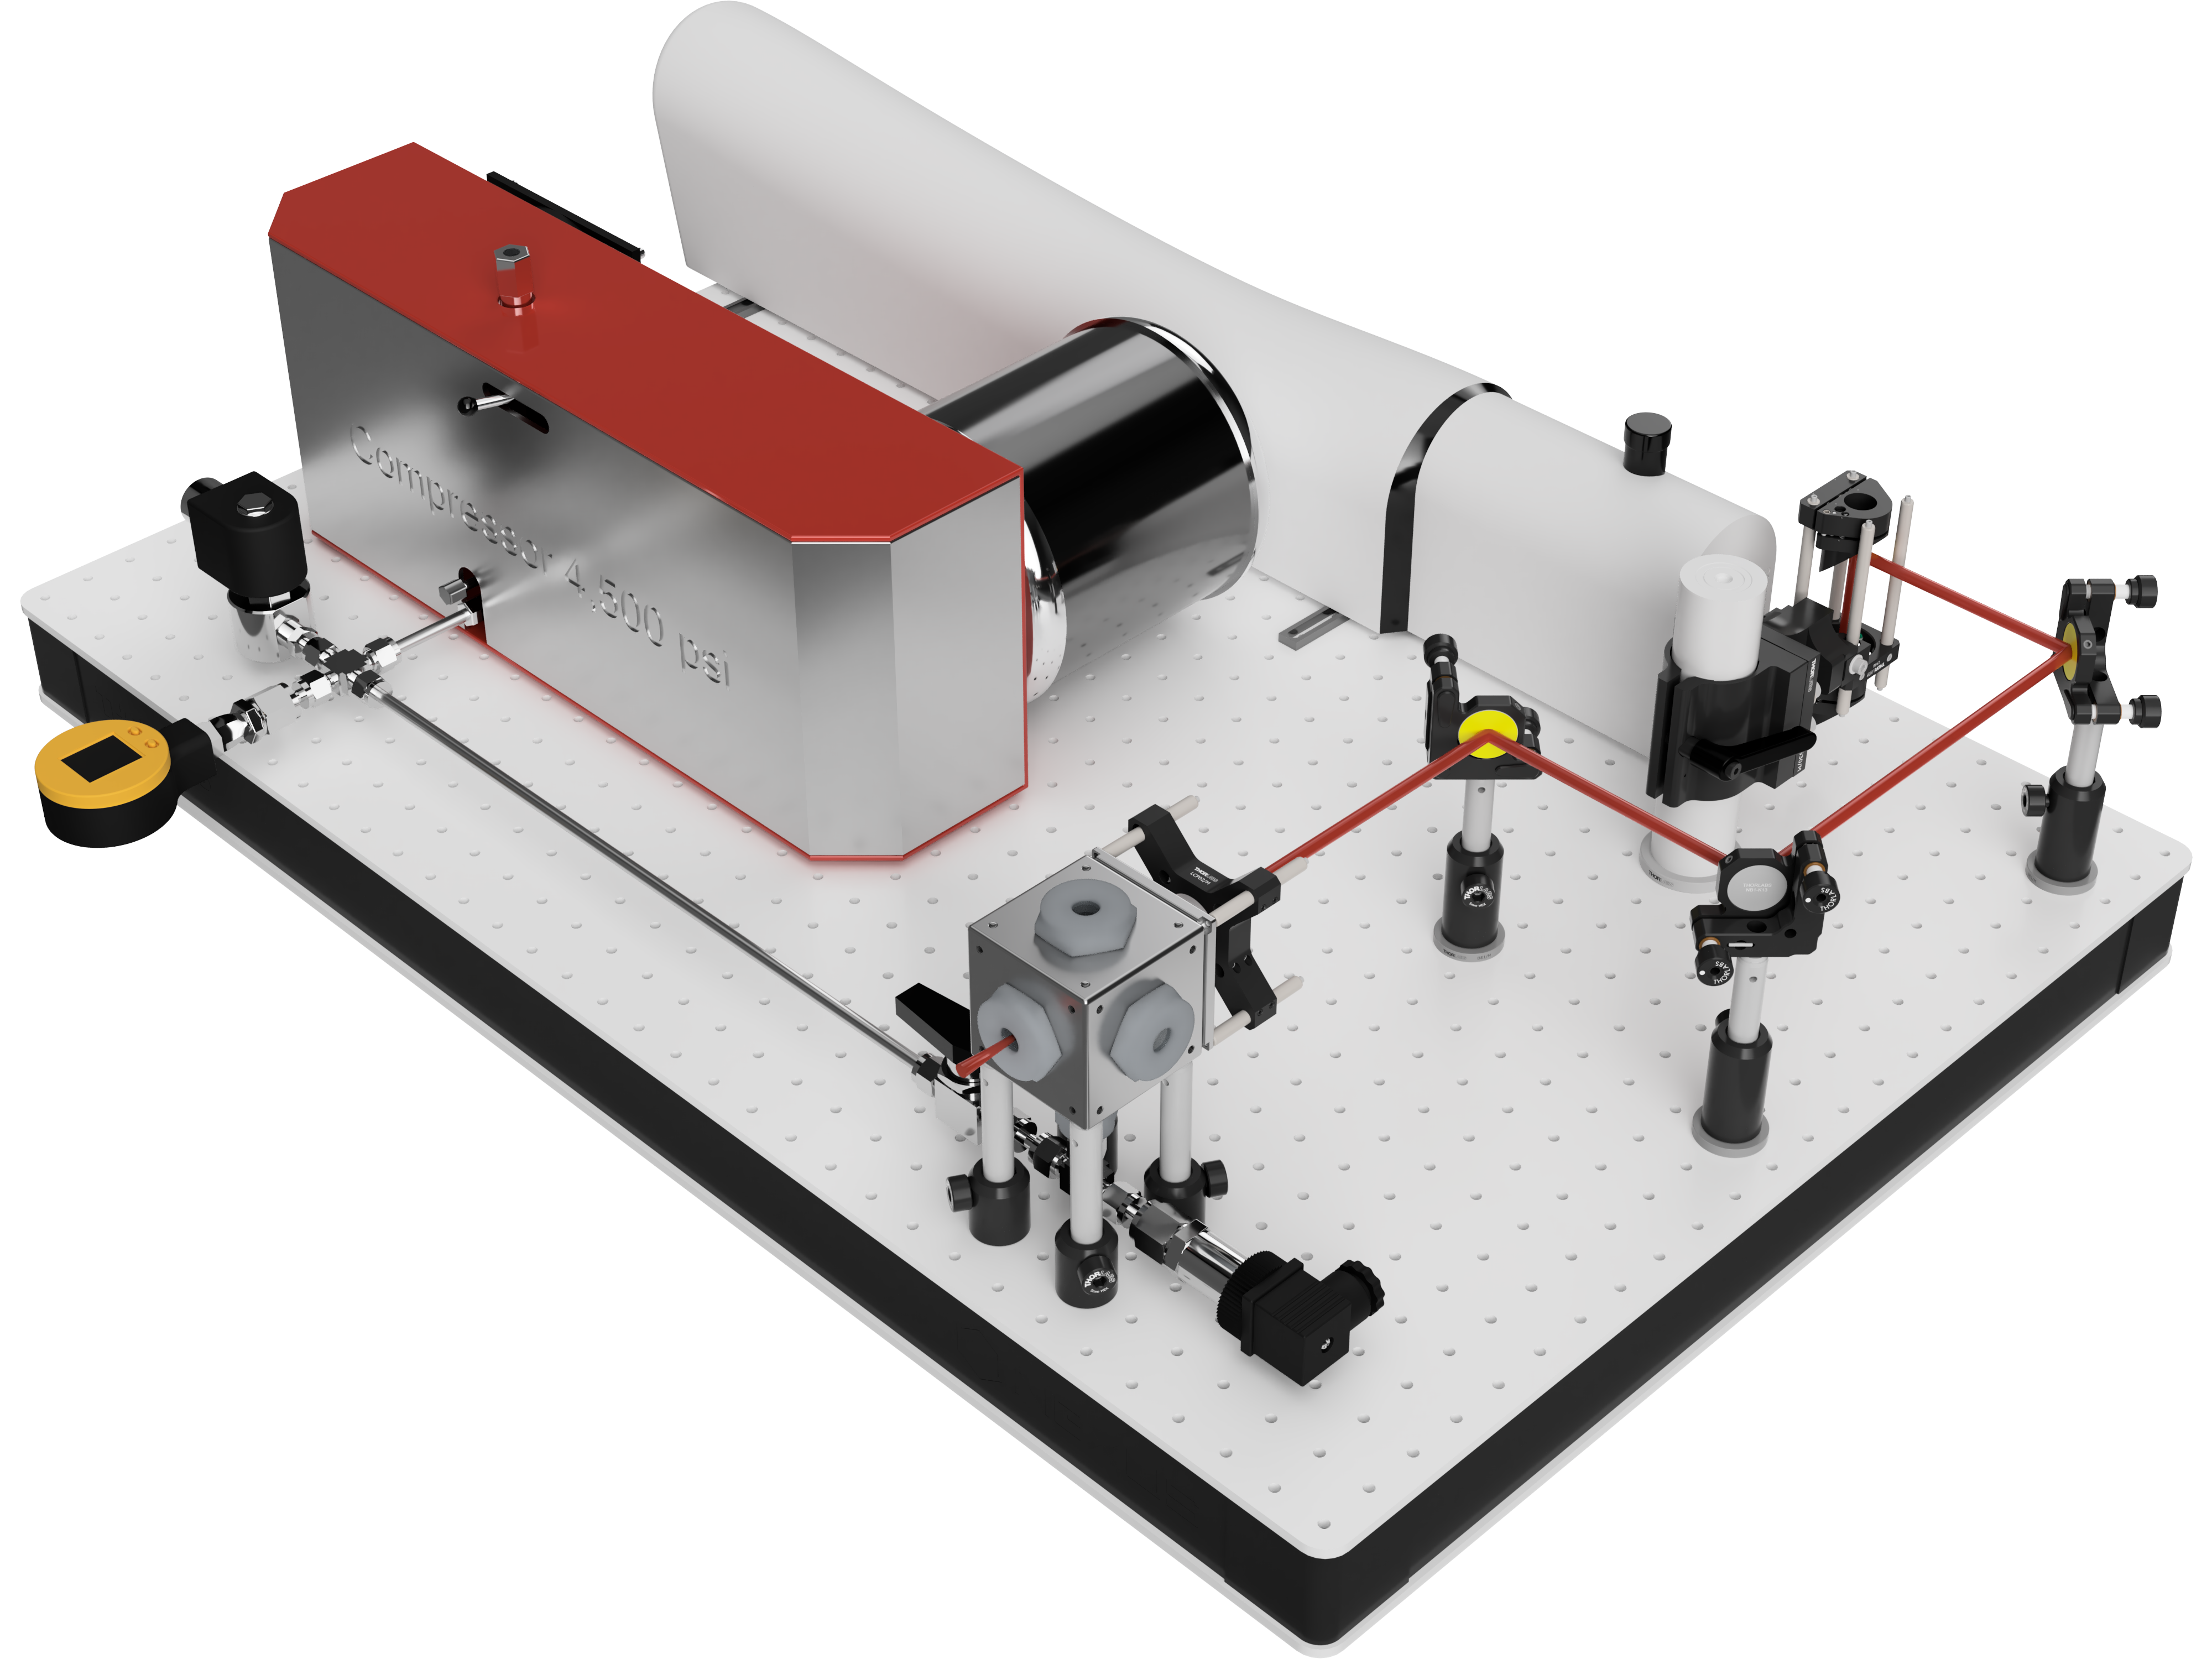
\includegraphics[width=130mm]{figures/ch2/setup/render.pdf}
\caption{Rendered image of experimental apparatus. A cube-shaped high-pressure chamber is located at the bottom of the middle of the image. In the image, Nd:YAG laser is placed, but an additional He-Ne laser is adopted in the same optical path for the diagnostic purpose. The three right-angle viewports are used to take a scattering image of droplets or interferograms. The same setup is utilized to generate laser produced plasma in the supercritical fluid which will be discussed in Chap.\ref{sec:ch4}. The images of plasma and light emission from plasma are also captured through side viewports. All the parts of the system are suitably selected to sustain the designed pressure safely and reliably.}
\label{fig:render}
\end{figure}

\begin{figure}[t!]
\centering
\includegraphics[width=100mm]{figures/ch2/phaseDiag/phaseDiag.pdf}
\caption{Extended phase diagram of homogeneous and equilibrium argon fluid. The red points on the graph represent the experimental conditions. The compressor has a working pressure of $300 \text{ bar}$. The argon fluid undergoes an adiabatic expansion to form the liquid droplets and clusters. The compressibility factor, which writes $Z=P/ρRT$, is unity for the case of an ideal gas. The NIST Chemistry WebBook provides information on argon's thermophysical characteristics \cite{linstorm2020nist}.}
\label{fig:phaseDiag}
\end{figure}

\begin{figure}[t!]
\centering
\includegraphics[width=130mm]{figures/ch2/droplet/imgProcess.pdf}
\caption{Image of the scattering signal from droplets with 2.5X magnification and their number counting. The image processing code for counting the number of droplets is not perfect but still reasonably perform. Note that 1 pixel corresponds to $4.8 ~\mathrm{\mu}\text{m}$, but the size measured in this image does not provide the actual size of the droplet due to the diffraction limit.}
\label{fig:imgProcess}
\end{figure}

A check valve (opening pressure: 300 bar) allows argon fluid to enter the high-pressure chamber from a reciprocating compressor. The compressor delivers roughly $6.8\text{ cm}^3$ of argon fluid per cycle (under the standard condition). The extended phase diagram of supercritical argon in Fig.\ref{fig:phaseDiag} \cite{linstorm2020nist, banuti2017similarity} shows a series of experiments along the line of red dots. Because the temperature is around two times above the critical temperature, spontaneous critical phenomena such as density fluctuations do not occur; yet, during compression, the fluid expands rapidly and adiabatically cools to form a liquid. When the argon fluid cools below 140 K, it experiences a phase transition, resulting in the formation of liquid droplets and clusters. The temperature drop of an expanding fluid is well understood (see \cite{hagena1981nucleation, chen2009pressure, tao2016revisiting}), and in Chap.\ref{sec:ch2-3-1}, we compare our experimental results to the COMSOL Multiphysics simulations.

The imaging optics with the ICCD camera captures images and videos of droplets with two different magnifications (2.5X and 11X). The droplets are individually identified owing to their higher Rayleigh–Mie scattering intensity compared to the scattering intensity of the argon fluid and clusters in the background \ref{fig:imgProcess}. The number density and the mean size of droplets are obtained from the lower- and higher-magnification data, respectively. For the lower magnification, the incident He-Ne laser is modified to a beam sheet with a laser line generator (or Powell lens) having the thickness of $100 ~\mu\text{m}$, which is used to calculate the volume number density of droplets from the 2D imaging result. Note that the size of individual droplets cannot be measured by direct imaging because of the diffraction limit of the visible light (light source: 633 nm He–Ne laser). Hence, Brownian motion analysis is adopted to determine the mean size of the droplets.



%----------------------------------------------------------------------------------------------------
\section{Formation of droplets and clusters}
\label{sec:ch2-3}

%----------
\subsection{Temperature drop of expanding fluids}
\label{sec:ch2-3-1}

We perform fluid/heat transport models (using the multiphysics modeling tool COMSOL) and compare them to the results to show that the expanding argon fluid achieves a low enough temperature to become a liquid. A thermocouple with a finite heat capacitance may not experience noticeable cooling since the compressor only delivers a tiny amount of fluid per cycle. As a result, we devised a temperature measurement system that involved filling a small buffer chamber with 300 bar of argon fluid and then abruptly purging it to record the temperature reduction using a thermocouple. The experimental data for the temperature profile along the axis are shown in Fig.\ref{fig:comsolSolenoid}, along with a comparison to simulations. The thermocouple is set $20-60 \text{ mm}$ away from the valve exit in the experiment. To compare with the experiment, each simulation result is averaged spatially inside the red dashed area and temporarily for $0-200 \text{ ms}$.

\begin{figure}[t!]
\centering
\includegraphics[width=130mm]{figures/ch2/comsol/comsolSolenoid.pdf}
\caption{A temperature drop of an expanding fluid through the solenoid valve from a buffer chamber and comparing the experimental results with the COMSOL Multiphysics simulations. The argon fluid of $300 \text {bar}$ filled in the buffer chamber suddenly expands into the air through the solenoid valve, and the thermocouple monitors the minimum temperature reached. \textbf{a,} The buffer chamber with 300 bar suddenly expands to an open space having 1 bar. \textbf{b,} The experimental measurement is compared with the time- and space-averaged temperature in the simulation results (0-200 ms, red dashed area). The error bands are the standard deviations of each point.}
\label{fig:comsolSolenoid}
\end{figure}

\begin{figure}[t!]
\centering
\includegraphics[width=130mm]{figures/ch2/comsol/comsolCompressor.pdf}
\caption{A temperature drop of an expanding fluid through the check valve of the compressor by COMSOL Multiphysics simulations. \textbf{a,} A set of simulations shows the fluid expansion through the check valve of the compressor outlet to the pipe connecting to the main chamber as a function of the initial pipe pressure. \textbf{b,} Minimum temperatures for different pipe pressures. The error bands are the standard deviations of each point.}
\label{fig:comsolCompressor}
\end{figure}

Another set of simulations depicts the temperature profile as the fluid expands abruptly through the compressor's check valve and then into the pipe connecting the main chamber (Fig.\ref{fig:comsolCompressor}). As the original pipe pressure rises, the gradient of the temperature profile reduces. For instance, Fig.\ref{fig:comsolCompressor}b shows the minimum temperature reached within the simulation volume by varying the pipe ($z>0$) pressure. When the pipe pressure is below 100 bar, the fluid cools to the point where it can form a liquid, which corresponds to the creation of droplets and clusters shown in Fig.\ref{fig:numdens}a and Fig.\ref{fig:opacity}a.

Because of heat conduction at the pipe surface, the overall temperature inside the chamber remains unaltered from ambient temperature despite the low local fluid temperature. Using the simplified dimensions of the stainless steel pipe ($r∼2 \text{ mm}$, $l∼800 \text{ mm}$, and $d∼10 \text{ mm}$, where $r$, $l$, and $d$ are the inner diameter, the total length, and the thickness of the pipe, respectively) and the thermal conductivity of a stainless steel $k \sim 16 \text{ W m}^{-1}\text{K}^{-1}$ and assuming the temperature difference between the inside and outside of the pipe $\delta T \sim 10 \text{ K}$, the heat transfer rate becomes
\begin{equation}
\frac{d Q}{d t} \sim k \left( \frac{2 \pi r l}{d} \right) \delta T \sim 160 \text{ W}
\end{equation}
In the experiment, the compressor delivers $N_1 \sim 2.7 \times 10^{-4} \text{ mol} \cdot \text{cycle}^{-1}$, and operates in $f \sim 4.1 \text{ Hz}$. Thus, the number of particles compressed into the chamber per unit time is $N = N_1 \cdot f \sim 1.1 \times 10^{-3} \text{ mol} \cdot \text{s}^{-1}$. Considering the power required to raise the temperature of such fluid from $100$ to $300 \text{ K}$,
\begin{equation}
P_{\text {heat}}=\bar{C}_{\text{P}} N \Delta T \sim 5.5 \text{ W}
\end{equation}
where the average heat capacitance $\bar{C}_{\text{P}} \sim 25 \text{ J K mol}^{-1}$ within the given temperature range under $10 \text{ bar}$ \cite{linstorm2020nist}. The conductive heat transfer rate through the pipe is much faster than the heating power, allowing the chamber to maintain a constant temperature. In the COMSOL simulation, this conclusion is also validated. Further compression to higher pressure increases convective heat transport, which helps keep the temperature of the fluid in the chamber.

%----------
\subsection{Number density of droplets}
\label{sec:ch2-3-2}

\begin{figure}[ht!]
\centering
\includegraphics[width=100mm]{figures/ch2/droplet/numdens.pdf}
\caption{Production of droplets. \textbf{a,} The number density of droplets generated by the continual compression of argon fluid in the high-pressure chamber. The droplet number density does not increase as the pressure exceeds $100 \text{ bar}$ because the temperature drop is not large enough to form a liquid at a higher chamber pressure (i.e., a smaller pressure difference between the chamber and check valve) and the droplets evaporate. The number density of droplets decreases due to evaporation in the medium. \textbf{b,} The compression rate by time. There is a competition between the generation and evaporation of droplets, as a finite time is required to raise the chamber pressure.}
\label{fig:numdens}
\end{figure}

In terms of droplet density, average lifetime of droplets, and medium opacity, Fig.\ref{fig:numdens}, \ref{fig:lifetime}, and \ref{fig:opacity} shows how SCF properties change as pressure increases. The substantial changes in these properties across the critical pressure are worth noting. The abrupt increase in droplet density over the critical pressure, above which it is saturated, is depicted in Fig.\ref{fig:numdens}a. Through the check valve, argon gas is cumulatively compressed into the chamber, forming liquid droplets and clusters. As the chamber pressure rises, the droplet creation rate falls, and droplet formation eventually ceases. It is consistent with the COMSOL simulation results – a sufficient temperature drop to form a liquid during a sudden expansion occurs when the chamber pressure is below $100 \text{ bar}$ (Fig.\ref{fig:comsolCompressor}b). The droplets formed during compression evaporate within the fluid as well. The number density of droplets does not keep increasing throughout the compression, as shown in Fig.\ref{fig:numdens}a. Instead, the generation and evaporation of the droplets co-occur and compete, and finally, above $100 \text{ bar}$, evaporation dominates.

%----------
\subsection{Lifetime of droplets}
\label{sec:ch2-3-3}

\begin{figure}[ht!]
\centering
\includegraphics[width=100mm]{figures/ch2/droplet/evaporation.pdf}
\caption{Lifetime of droplets. \textbf{a,} The evaporation timescale of the droplets at different pressures. The evaporation timescale of LL droplets exceeds two hours below the critical pressure and suddenly decreases to an hour above the critical pressure. Again, the evaporation timescale is extended with increasing pressure above the critical pressure. \textbf{b,} Exponential decrease of the droplet's number density. The number density of the droplets decreases as time goes, and the characteristic lifetime is defined when the density reaches below $1/10$th of the initial value.}
\label{fig:lifetime}
\end{figure}

At varied chamber pressures, the lifetime of droplets or the evaporation timescale (defined by the period when the droplet number density becomes $1/10\text{th}$ of the maximum) is illustrated in Fig.\ref{fig:lifetime}a. The droplet number density is monitored for two hours after compression for each pressure condition. The evaporation timeframe decreases and eventually increases when the chamber pressure is increased above the critical pressure. We use the evaporation model and the consequent cluster effect to explain both the abrupt change at the critical pressure and the monotonic ascent at higher pressures in Chap.\ref{sec:ch2-5}.

%----------
\subsection{Existence of clusters}
\label{sec:ch2-3-4}

\begin{figure}[ht!]
\centering
\includegraphics[width=130mm]{figures/ch2/cluster/opacity.pdf}
\caption{Opacity analysis for the existence of the nanometer-sized clusters. \textbf{a,} Opacity of the high-pressure chamber while compressing. It is not sufficient to obtain such opacity with the droplets only. \textbf{b,} Refractive index for the LL clusters and droplets. The refractive index for LL argon fluid packages is assumed to be that of the liquid argon at about $100 \text{ K}$. \textbf{c,} Expected number density and size of the clusters to satisfy the opacity measurement. The gray shaded area is forbidden because the number of atoms exceeds the total number of atoms for the given chamber conditions ($100 \text{ bar}$, $294 \text{ K}$). The clusters should have density and size within the yellow shaded area. The dark-blue dot corresponds to the opacity for the case of atoms only (i.e., no clusters).}
\label{fig:opacity}
\end{figure}

The opacity inside the chamber rapidly increases, such as in Fig.\ref{fig:opacity}, which we attribute to the formation of a significant number of clusters. It is worth noting that these clusters are created by a compression-expansion process rather than by critical phenomena.

Clusters, unlike drops, are too tiny to be distinguished separately. They increase the medium opacity through the Rayleigh scattering and absorption. To ensure that these clusters, not the droplets, are responsible for the majority of the opacity, we calculate the opacity due to particle scattering as follows:
\begin{equation}
\chi \left( \lambda \right) = \sum_{\text{s}} n_{\text{s}} \sigma_{\text{s}} \left( \lambda \right)
\end{equation}
where $n_\text{s}$ and $\sigma_\text{s}$ are the number density and the total scattering cross-section of the particle species s (droplets, clusters, and atoms), respectively \cite{fivsak2016rayleigh, hulst1981light, howell2020thermal}, and $\lambda$ is the wavelength of the incident light. For a large particle with a size comparable to $\lambda$, $\sigma \sim \pi r^2$ where $r$ is the mean radius of the particles. The upper limit of the opacity caused by the droplets is about $0.002 \text{ mm}^{-1}$ (using $n_\text{d} \sim 2500 \text{ mm}^{-3}$ around $150 \text{ bar}$ and $r_\text{d} \sim 0.5 \times 10^{-3} \text{ mm}$, see Fig.\ref{fig:numdens} and \ref{fig:size}), which is quite small, implying that the major contribution to opacity comes from the clusters and not from the droplets.

The Rayleigh scattering cross-section of a small particle with radius $r$ is
\begin{equation}
\sigma = \frac{2 \pi}{3} \frac{\left( 2 r \right)^{6}}{\lambda^{4}}\left( \frac{n^{2}-1}{n^{2}+2} \right)^{2}
\end{equation}
where $\lambda$ is the wavelength of the incident light and n is the refractive index ratio between the particle and a medium \cite{howell2020thermal}. The criteria of cluster size and number density required to attain such opacity are shown in Fig.\ref{fig:opacity}c. The gray area is  where the mass conversation is violated for the given condition ($100 \text{ bar}$, $294 \text{ K}$). A cluster is assumed to have $n \sim 1.2$ – the value for a liquid argon at about $100 \text{ K}$ \cite{hanna2010equation}. To explain the measured opacity, the cluster conditions should be in the yellow highlighted area. The chamber opacity for the situation of ``atoms only'' is nowhere near the experimental result (note the dark-blue point in Fig.\ref{fig:opacity}). As a result, the clusters are the primary cause of the medium's fogginess and opacity.

As we will see later, a large number of clusters in the argon fluid have a significant impact on mass transfer at the droplet surface. In addition, the evaporation timescale of the droplets is affected by the clusters in the SCF.


%----------------------------------------------------------------------------------------------------
\section{Brownian motion analysis}
\label{sec:ch2-4}

%----------
\subsection{Droplet size}
\label{sec:ch2-4-1}

\begin{figure}[ht!]
\centering
\includegraphics[width=100mm]{figures/ch2/Brownian/size.pdf}
\caption{Mean size of droplets at different pressures. \textbf{a,} The mean size at each pressure is calculated using Brownian motion analysis. The motions of the droplets are divided into two axes, yielding two sets of one-dimensional displacements. With the emergence of the clusters, the medium viscosity tends to decrease. The green dashed line shows the difference in anticipated droplet sizes when the cluster effect on viscosity is taken into consideration in a condition with a high cluster density, as in our experiments. The error band shows $90\%$ confidence interval of normal distribution fit for each pressure. \textbf{b-c,} The histograms show the displacement of droplets during the elapsed time ($0.02 \text{ s}$) and their normal distribution fits at $100 \text{ bar}$ and $250 \text{ bar}$, respectively.}
\label{fig:size}
\end{figure}

Visual inspection of the argon SCFs reveals a large number of submicron-sized droplets. The droplets, in particular, persist for a long time, allowing us to measure the size using direct imaging and Brownian motion analysis.

Brownian particles floating in argon fluid are used to calculate the average size of droplets. High-resolution imaging optics (11X magnification) and ICCD track the small displacements of droplets caused by their jiggling motion (50 frames per second). The videos are taken three minutes after compression, allowing any turbulence in the medium to be stabilized at each operating pressure. 

The mean squared displacement $\sigma^2$ of Brownian particles for one-dimensional motion is expressed by the following equation \cite{einstein1956investigations}:
\begin{equation}
\sigma^2 = 2Dt
\end{equation}
where $D$ is the diffusion coefficient of the surrounding medium and t is the elapsed time (in our experiment, $t=0.02 \text{ s}$). The Stokes-Einstein equation relates the diffusion coefficient to the mean radius $r$ of the Brownian particles \cite{einstein1956investigations}:
\begin{equation}
D=\frac{k_\text{B} T}{6\pi \eta r}
\label{eq:einstein}
\end{equation}
where $k_\text{B}$, $T$, and $\eta$ are the Boltzmann constant, the temperature, and the dynamic viscosity of the surrounding medium, respectively. We referred to the NIST Chemistry WebBook \cite{linstorm2020nist} for the dynamic viscosity of argon at each pressure. The mean radius of the droplets, based on the dynamic viscosity, varies from about $250$ to $400 \text{ nm}$ depending on the final chamber pressure, as shown in Fig.\ref{fig:size}a. Using a homogeneous medium viscosity, on the other hand, may introduce errors in size estimation if the medium contains a large number of clusters. This is because when some portions of the medium are clustered, the viscosity is lower than when the medium is homogeneous, resulting in underestimating the droplet size. In Chap.\ref{sec:ch2-4-2}, we will go over this in more detail.

%----------
\subsection{Viscosity correction for a clustered medium}
\label{sec:ch2-4-2}

The size estimation by the Brownian motion analysis obtained through Eq.\ref{eq:einstein} depends on the accuracy of the medium viscosity. We used the viscosity value for a homogeneous argon fluid at the given pressure and temperature from the NIST Chemistry WebBook \cite{linstorm2020nist} in our calculations. However, as the pressure rises, more clusters form in the medium, and it is crucial to understand how this affects the fluid's viscosity. Therefore, instead of a comprehensive viscosity analysis, a simplified analysis will suffice to show that the viscosity of the clustered medium will be lower than that of the homogeneous medium.

According to the kinetic model, the viscosity $\eta$ of a medium consisting of spherical particles of radius $r$ and mass $m$ is
\begin{equation}
\eta \propto \frac{\sqrt{m T}}{\pi r^{2}}
\end{equation}
where $T$ is the temperature of the medium \cite{chapman1990mathematical}. The proportionality constant may be temperature dependent when considering particle interaction, but the fundamental relationship does not change significantly. Assume that each cluster has an average of $N$ argon atoms and that the temperature is constant, the proportionality of the viscosity writes
\begin{equation}
\eta \propto N^{-1 / 6}
\end{equation}
as $m \propto N$ and $r \propto N^{1/3}$. As a result, if atoms aggregate to form clusters, the viscosity of the medium decreases, and the droplet size is underestimated for a higher cluster density. The green dashed curve in Fig.\ref{fig:size} illustrates the cluster effect on droplet size estimation.

In conclusion, we show that droplets can survive for long periods in SCF. However, according to the analysis of mass transport, the clustering effect can reduce the lifetime of droplets, implying that the clustering effect is crucial to understanding non-equilibrium thermodynamic processes in supercritical states.

The existence of quasi-steady clusters and droplets will have practical implications in planetary meteorology, power plant cooling systems, pharmaceutical processes, high-power switching, and high-pressure fuel injection, among other fields of science and engineering involving SCFs. Clusters and droplets, for example, may have an impact on mass transport processes in Venus' and Jupiter's dense atmospheres. In the recent development of the SCF CO2 cleaning technique in semiconductor fabrication, the same effect may have to be considered. Our findings are expected to be a turning point in studying SCFs' non-equilibrium, transient behavior. The physics that supports clusters and droplets in SCFs will be a widespread issue in various engineering problems involving heat and momentum transport processes in SCFs.

%----------
\subsection{Size distribution}
\label{sec:ch2-4-3}

The Brownian motion analysis provides the size of the droplets, and we might be wondering how the calculation will be affected if the size distribution changes. For the brief answer, this analysis gives the average of any size distribution. That is to say, with this statistical analysis, the distribution information is screened, and only the average of particular size distribution remains. Thus, technically, the radius from Eq.\ref{eq:einstein} represents the `arithmetic mean' of the size distribution.

\begin{figure}[ht!]
\centering
\includegraphics[width=100mm]{figures/ch2/Brownian/distributionEffect.pdf}
\caption{Four different artificially designed distribution functions and their resulting particle displacements distributions. \textbf{a,} The functions follow the normal distributions with different parameters ($f_1$, $f_2$, and $f_3$), or combination of two normal distributions ($f_4$). The mean of function $f_4$ is set to be the same with that of functions $f_2$ and $f_3$ \text{b,} The resulting displacements distributions from each size distributions. The physical values -- $T=294 \text{ K}$ and $\eta \sim 2.53\times10^{-5} \text{ Pa}\cdot\text{s}$ are used to append the units of the order of the experimental results.}
\label{fig:distributionEffect}
\end{figure}

\begin{table}[h!]
\footnotesize
\centering
\begin{tabular}{c|cccc}
                    & $f_1$   & $f_2$   & $f_3$  & $f_4$   \\ \hline
$m_r$          & 150     & 300    & 300    & 300 \\
$\sigma_r$   & 30.0    & 30.0    & 55.1    & 54.8 \\
$\sigma_x$  & 2.28    & 1.14    & 1.14    & 1.14
\end{tabular}
\caption{Statistical information of distribution functions. The four functions have the different mean size $m_r$, the standard deviation of size $\sigma_r$, and the resulting standard deviation of displacements of Brownian particles $\sigma_x$. The standard deviations of displacements follow the mean size and are not affected by the shape of the original distribution function.}
\label{table:standardDeviation}
\end{table}

To check how the size distribution of particles contributes to the Brownian motion analysis, we introduce four artificially designed distribution functions having different means and standard deviations (Fig.\ref{fig:distributionEffect}a):
\begingroup
\allowdisplaybreaks
\begin{align}
f_1 &= C_1 e^{ - \frac{1}{2} \left( \frac{r - 150}{30} \right)^2 } \\
f_2 &= C_2 e^{ - \frac{1}{2} \left( \frac{r - 300}{30} \right)^2 } \\
f_3 &= C_3 e^{ - \frac{1}{2} \left( \frac{r - 300}{55} \right)^2 } \\
f_4 &= C_4 \left[ e^{ - \frac{1}{2} \left( \frac{r - 250}{10} \right)^2 } + e^{ - \frac{1}{2} \left( \frac{r - 350}{30} \right)^2 } \right]
\end{align}
\endgroup
, where $C_1$ through $C_4$ are the normalization factors. For each size distribution, the displacement distribution is retrieved (Fig.\ref{fig:distributionEffect}b). In other words, the displacements of virtual particles where the population distribution follows the given functional form are calculated. As in the Table. The standard deviation of the displacements of virtual Brownian particles is decided by the mean of the original distribution function and is not affected by the original function's shape. This shows that the Brownian motion analysis only gives the mean size of the particles and tells nothing about the size distribution.



%----------------------------------------------------------------------------------------------------
\section{Modified evaporation model}
\label{sec:ch2-5}

The estimated droplet radii trend around the critical pressure (Fig.\ref{fig:size}a) appears to conflict with the droplet lifetime (evaporation timescale) trend (Fig.\ref{fig:lifetime}a). Thus, smaller droplets below the critical pressure may take longer to evaporate than larger droplets above the critical pressure, based on the two trends. Consider the effect of clusters on mass transport at the droplet surface to resolve this apparent contradiction.

\begin{figure}[t!]
\centering
\includegraphics[width=100mm]{figures/ch2/transport/evaporation.pdf}
\caption{Graphical illustration of the mass transport at a droplet surface. The emergence of clusters reduces the mass influx, and consequently, the evaporation time of a droplet decreases. The mass carriers of the influx and outflux are assumed to be clustered, altering the number of particles within a given time interval to be transferred into- or out of- the transition layer.}
\label{fig:evaporation}
\end{figure}

It is impractical to consider all of the interactions between the atoms in a submicron-sized droplet in a dense background fluid to calculate the evaporation timescale. On the other hand, a submicron-sized droplet is large enough to consider evaporation as a surface process. To explain our experimental results, we use an evaporation model similar to that of subcritical fluids \cite{ishiyama2004molecular, julin2013mass}.

The droplet and the surrounding fluid are in a quasi-thermal equilibrium over an hour, implying that mass influx $\Gamma_\text{in}$ would balance mass outflux $\Gamma_\text{out}$ in the transition layer around the droplet surface (illustrated in Fig.\ref{fig:evaporation}), and suggesting that the net mass flux $\Gamma_\text{net}$ is negligible:
\begin{equation}
\begin{aligned}
\Gamma_{\text{net}} &= \Gamma_{\text{out}} - \Gamma_{\text{in}} \\
&= v_{\text{out }} \rho_{\text{out}} - v_{\text{in }} \rho_{\text{in}} \approx 0
\end{aligned}
\end{equation}
where $v_\text{in(out)}$  and $\rho_\text{in(out)}$ are the surface-normal mean velocities and mass densities, respectively. The outflux is defined as the flux leaving the inner boundary of the transition layer, i.e., the surface of the droplet. The surface-normal mean velocity is then
\begin{equation}
v_{\text {in }(\mathrm{out})}=\sqrt{\frac{8 k_{\mathrm{B}} T}{\pi m_{\mathrm{in}(\mathrm{out})}}}
\end{equation}
where $m_\text{in(out)}$ denotes the mass of the mass carrier. Assuming that the droplet has the density of liquid argon  ($\rho_\text{out} = \rho_\text{droplet} = \rho_\text{liquid}$), the net mass flux becomes
\begin{equation}
\Gamma_{\mathrm{net}} \approx \sqrt{\frac{8 k_{\mathrm{B}} T}{\pi}}\left(\frac{\rho_{\text {droplet }}}{\sqrt{m_{\text {out }}}}-\frac{\rho_{\text {medium }}}{\sqrt{m_{\text {in }}}}\right)
\end{equation}
where the mass density of influx $\rho_\text{in} = \rho_\text{medium}$. The evaporation timescale would be prolonged if the net flux remained insignificant.

When the critical pressure is crossed, the number of clusters in the medium suddenly rises, as shown in Fig.\ref{fig:opacity}a, and the average mass of the mass carrier of the particle influx $m_\text{in}$ increases. As a result, the influx is lowered substantially, and the evaporation period is shortened (see the region around the critical pressure in Fig.\ref{fig:lifetime}a). On the other hand, the number of clusters is less at subcritical pressures, thus the influx is greater, resulting in a considerably longer evaporation period (the higher pressure condition in Fig.\ref{fig:lifetime}a). If the pressure rises to the point where it surpasses the critical pressure, the number of clusters increases as well. However, as $\rho_\text{medium}$ gradually approaches $\rho_\text{droplet}$, the overall flux is rebalanced, resulting in a prolonged evaporation timescale.
 % chapter 2 
%!TEX root = ../thesis.tex
% chapter 3

\chapter{Strongly coupled plasma}
\label{sec:ch3}

The plasma in which the Coulomb potential energy of the system exceeds the thermal kinetic energy of the particles is called the strongly coupled plasma (SCP). The Coulomb coupling parameter of plasma is defined as
\begin{equation}
\begin{aligned}
\Gamma &= \frac{U}{K}=\frac{e^{2} / 4 \pi \varepsilon_{0} R_\text{WS}}{k_\text{B} T_{e}} \\
&=\left(\frac{e^{2}}{4 \pi \varepsilon_{0} k_\text{B} T_{e}}\right)\left(\frac{4 \pi n_{e}}{3}\right)^{1 / 3}
\end{aligned}
\end{equation}
, where $U$ and $K$ are average coulomb potential and kinetic energy of an electron, and $e$, $\varepsilon_0$, $k_\text{B}$, $R_\text{WS}$, $T_e$, and $n_e$ are electron charge, vacuum permeability, Boltzmann constant, Wigner-Seitz radius, electron temperature and electron density, respectively. Technically SCP satisfy $\Gamma \geq 1$. Standard theories for an ideal plasma fail to describe such conditions of strongly correlated systems \cite{stanton2016ionic}. The SCPs are found in many objects such as stars, galaxies, white dwarf stars, cores of Jovian planets \cite{ichimaru1982strongly}, lightening in the thick planetary atmospheres \cite{cartier2020planetary}, and inertial confinement fusion \cite{remington2006experimental}, bringing both scientific and technical interests. Owing to their theoretical and practical importance, a great amount of efforts was dedicated for a few decades.



%----------------------------------------------------------------------------------------------------
\section{Physical regimes}
\label{sec:ch3-1}

The plasmas can be classified within the phase diagram consisting of temperature and density of electrons. Strongly coupled dense plasmas span a wide range of unfamiliar regime having high density and relatively low temperature (Fig.\ref{fig:taxonomy}). Due to the close proximity of ions, SCP exhibits the features of condensed matter. Both theories on the classical (ideal) plasma physics and condensed matter (quantum) physics are required to understand such plasmas. In addition to the coupling parameter $\Gamma$, there are several more parameters for defining which region the plasma corresponds to and what kind of theories should be applied according to the electron temperature and density, such as Debye number $N_\text{D}$, energy density $P$, and degeneracy paramter $\Theta$.

%----------
\subsection{Assumptions for ideal plasma}
\label{sec:ch3-1-1}

For an ideal plasma, the Debye length $\lambda_\text{D}$ is the nominal shielding length of a charged particle. A particle outside the Debye sphere with radius of Debye length do not "feel" the coulomb potential. The Debye number $N_\text{D}$ is the number of electrons in the Debye sphere. The concept of Debye shielding is achieved from a circular logic for an ideal plasma. The two assumptions that the collisions between particles are negligible and that $N_\text{D}$ is sufficiently large guarantee each other, and only in that case the Debye shielding is valid \cite{bellan2008fundamentals}.

\begin{figure}[ht!]
\centering
\includegraphics[width=100mm]{figures/ch3/Debye/shielding.pdf}
\caption{Schematic diagram for the Debye shielding. As the charge of the test particle is gradually introduced, the surrounding field particles move to cancel out the electrostatic potential.}
\label{fig:DebyeShielding}
\end{figure}

The Debye length is obtained from the following three relations: Boltzmann relation, Poisson equation, and charge neutrality. First, let us consider the Boltzmann relation starting with the equation of motion for each species s
\begin{equation}
m_\text{s} \frac{d \vec{v}_\text{s}}{d t} = -q_\text{s} \nabla \phi - \frac{\nabla  p_\text{s}}{n_\text{s}}
\label{eq:EOM}
\end{equation}
, where $\vec{v}_\text{s}$ and $p_\text{s}$ are the velocity and pressure for the species s. The omitted terms in the above equation are as follows: 1. the Lorentz force $q \vec{v} \cross \vec{B}$, 2. vector potential in the electric field $\vec{E} = -\nabla \phi - \partial \vec{A} / \partial t$, 3. collision (friction) force $\vec{R}_f$, and 4. viscosity. What assumptions make it possible to exclude these terms? There are four assumptions: 1. negligible magnetic field ($q \vec{v} \cross \vec{B} \approx 0$), 2. slow transition ($\partial \vec{A} / \partial t \approx 0$), 3. collisionless plasma (no friction and no viscosity), and 4. well defined temperature (the particle for each species are in thermal equilibrium among themselves and their energy distribution follows the Maxwellian distribution function). The pressure gradient term is approximated as 
\begin{equation}
\begin{aligned}
\nabla p_\text{s} &= k_\text{B} T_\text{s} \nabla n_\text{s} + n_\text{s} \nabla \left( k_\text{B} T_\text{s} \right) \\
&= k_\text{B} T_\text{s} n_\text{s} \left( \frac{\nabla n_\text{x}}{n_\text{s}} + \frac{\nabla T_\text{s}}{T_\text{s}} \right) \\
&\approx k_\text{B} T_\text{s} \nabla n_\text{s}
\end{aligned}
\end{equation}
, when $\nabla n/n \gg \nabla T/T$ by assuming the temperature gradient is very small. From the slow transition approximation, the Eq.\ref{eq:EOM} becomes
\begin{equation}
- q_\text{s} \nabla \phi - \left( \frac{k_\text{B} T_\text{s} \nabla n_\text{s}}{n_\text{s}} \right) \approx 0
\end{equation}
When $\phi \left( \vec{r} \right)$ and $T_\text{s} \left( \vec{r} \right)$ are spatially uniform, we get the Boltzmann relation
\begin{equation}
n_\text{s} \left(\vec{r} ~\right) = n_\text{s0} \left( \vec{r} ~\right) \exp \left[ \frac{-q_\text{s} \phi \left( \vec{r} ~\right)}{k_\text{B} T_\text{s} \left( \vec{r} ~\right) }\right]
\label{eq:BoltzmannRelation}
\end{equation}
If the potential energy is much smaller than the kinetic energy, i.e. $\abs{q_\text{s} \phi / k_\text{B} T}\ll 1$, the Eq.\ref{eq:BoltzmannRelation} simplifies to 
\begin{equation}
n_\text{s} \left(\vec{r} ~\right) \approx n_\text{s0} \left( \vec{r} ~\right) \left[ 1- \frac{q_\text{s} \phi \left( \vec{r} ~\right)}{k_\text{B} T_\text{s} \left( \vec{r} ~\right) }\right]
\label{eq:BoltzmannRelationApprox}
\end{equation}
The relations to consider next are the Poisson equation and the charge neutrality:
\begin{equation}
\begin{aligned}
\nabla \cdot \vec{E} &= - \nabla^2 \phi \\
&= \frac{\rho}{\varepsilon_0} \\
&= \frac{q_\text{T} \delta \left( \vec{r} ~\right) +\sum_\text{s} q_\text{s} n_\text{s} \left( \vec{r} ~\right)}{\varepsilon_0}
\end{aligned}
\label{eq:Poisson}
\end{equation}
\begin{equation}
\sum_\text{s} q_\text{s} n_\text{s,o} = 0
\label{eq:chargeNeutral}
\end{equation}
, where $q_\text{T}$ is the charge of the test particle and $\rho$ is the total charge density.
By plugging the Eq.\ref{eq:BoltzmannRelationApprox} and \ref{eq:chargeNeutral} into the \ref{eq:Poisson}, we get
\begin{equation}
- \nabla^2 \phi = \frac{q_\text{T}}{\varepsilon_0} \delta \left( \vec{r} ~\right) - \sum_\text{s} \left( \frac{n_\text{s0} q_\text{s}^2}{\varepsilon_0 k_\text{B} T_\text{s}} \right) \phi
\label{eq:PoissonApprox}
\end{equation}
Let us define the Debye length of each species $\lambda_\text{s}$ as
\begin{equation}
\frac{1}{\lambda_\text{s}^2} \equiv \frac{n_\text{s0} q_\text{s}^2}{\varepsilon_0 k_\text{B} T_\text{s}}
\end{equation}
and the total Debye length $\lambda_\text{D}$ writes
\begin{equation}
\frac{1}{\lambda_\text{D}} \equiv \sum_\text{s} \left( \frac{1}{\lambda_\text{s}^2} \right)
\end{equation}
Now Eq.\ref{eq:PoissonApprox} becomes
\begin{equation}
- \nabla^2 \phi + \frac{1}{\lambda_\text{D}^2} \phi = \frac{q_\text{T}}{\varepsilon_0} \delta \left( \vec{r} ~\right)
\label{eq:PoissonApproxSimplified}
\end{equation}
Finding the spherical symmetric solution of the form
\begin{equation}
\phi=\frac{f(r) q_\text{T}}{4 \pi \epsilon_{0} r}
\end{equation}
, and note that the delta function writes 
\begin{equation}
\nabla^{2}\left(\frac{1}{r}\right)=-4 \pi \delta \left( \vec{r} \right)
\end{equation}
We get $f(0)=1$ and $f''(r)=f(r)/\lambda_\text{D}^2$ which leads the final solution 
\begin{equation}
\phi \left( \vec{r} ~\right) = \frac{q_\text{T}}{4 \pi \varepsilon_0 r} \exp \left( -\frac{r}{\lambda_\text{D}} \right)
\label{eq:shieldedPotential}
\end{equation}

The potential of the form of Eq.\ref{eq:shieldedPotential} is called in several names such as Yukawa potential, Debye-H\"{u}kel potential, or shielded Coulomb potential. Recalling that any particle could have been the test particle, the effective potential of any plasma particle is described with the Eq.\ref{eq:shieldedPotential}. Note that, this analysis is only valid when the number of charged particle within the shielding sphere with a radius $\lambda_\text{D}$ (called Debye number $N_\text{D}$) is large enough, i.e. $N_\text{D} = 4 \pi n_0 \lambda_\text{D}^3/3 \gg 1$. To conclude, for the ideal plasmas the Debye shielding and the collisionless nature are the interdependent conditions and both of which are valid only when the Debye number is large enough.

%----------
\subsection{Failure of Debye shielding}
\label{sec:ch3-1-2}

In the case of SCP with high electron density, the screening is not possible because the distance among the particles is small compared to the Debye length. If the Debye shielding concept predicted from the ideal plasma theory is simply expanded, we encounter $N_\text{D} < 1$ at some point. As discussed above, Debye shielding is only valid when a sufficient number of charged particles are guaranteed to exist.

\begin{figure}[ht!]
\centering
\includegraphics[width=130mm]{figures/ch3/Debye/number.pdf}
\caption{Simple extension of Debye shielding concept to a dense plasma. \textbf{a,} When the electron density increases, at some point, the inter-particle distance exceeds the Debye length. \textbf{b,} The Debye number drops below unity and the shielding assumption does not holds anymore. The cores of planets as well as the plasma generated in our experiment are under such condition.}
\label{fig:DebyeNumber}
\end{figure}

\begin{figure}[ht!]
\centering
\includegraphics[width=130mm]{figures/ch3/lowering/continuumLowering.pdf}
\caption{Graphical illustration of continuum lowering. When atoms are close together, the energy levels are distorted by adjacent neighbors and the valence electrons do not stay in the bound levels any more.}
\label{fig:continuumLowering}
\end{figure}

When the Debye shielding is not valid the energy levels of atoms are distorted by adjacent neighbors and the valence electrons may be released from the atoms (Fig.\ref{fig:continuumLowering}). This phenomenon is called continuum lowering and the plasma exhibits the features of liquid metal or condensed matter. The amount of continuum lowering for the strongly coupled plasma is \cite{griem1962high, bataller2014blackbody}
\begin{equation}
\Delta \chi = \frac{(\bar{Z}+1) e^{3}}{4 \pi \varepsilon_{0}} \sqrt{\frac{\bar{Z}(\bar{Z}+1) n_{0}}{\varepsilon_{0} k_{B} T_{e}}}
\label{eq:lowering}
\end{equation}
, where $\bar{Z}$ is the effective degree of ionization, $e$ is the electron charge, and $\varepsilon_0$ is the vacuum permittivity \cite{bataller2014blackbody, griem1962high}.

In such plasma, the electrons become degenerate as the Pauli exclusion principle comes in for the occupation of the free electron states and they start to follow Fermi-Dirac statistics \cite{murillo2004strongly}. A measure of the importance of degeneracy is given by the degeneracy parameter,
\begin{equation}
\Theta=\frac{T_{e}}{T_{F}}=\frac{2 m_{e} k_{B} T_{e}}{\hbar^{2}\left(3 \pi^{2} n_{e}\right)^{2 / 3}}
\end{equation}
, where $T_\text{F}$ is the Fermi temperature.
The regime corresponding to $\Theta \leq 1$ is shown as a shaded area with dark-red color on the top-left corner of Fig.\ref{fig:taxonomy}. When $\Theta \gg 1$, the electrons are considered to follow the classical Maxwell-Boltzmann statistics, and, for the other case, they follow Fermi-Dirac statistics.



%----------------------------------------------------------------------------------------------------
\section{Electron-ion collision}
\label{sec:ch3-2}

The energy relaxation from electron to ion is governed by
\begin{equation}
\frac{d \mathcal{E}_e}{d t}=-\nu_{Eei}\left(\mathcal{E}_{e}-\mathcal{E}_{i}\right)
\end{equation}
, where $\mathcal{E}_{e(i)}$ is the electron (ion) energy, and $\nu_{Eei}$ is the collision frequency of energy change from electron to ion. Note that, as the ion to electron mass ratio is very large, the orders of momentum or energy collision frequency between species are diverse (see Table.\ref{table:collFreq}). In this case, $\nu_{Eei} = \left( m_e/m_i \right) \nu_{ei}$.

\begin{table}[h!]
\footnotesize
\centering
\begin{tabular}{ccc}
\hline \hline
$\sim 1$        &   $\sim \left( m_e/m_i \right)^{1/2}$   &   $\sim m_e/m_i$   \\ \hline
$\nu_{ee}$     &   $\nu_{ii}$                                        &   $\nu_{ie}$             \\
$\nu_{ei}$      &   $\nu_{Eii}$                                      &   $\nu_{Eei}$           \\
$\nu_{Eee}$   &                                                          &   $\nu_{Eie}$            \\
\hline \hline
\end{tabular}
\caption{The orders of momentum or energy collision frequencies between electron between species \cite{bellan2008fundamentals}. The energy transfer frequency from electron to ion $\nu_{Eei}$ is smaller from momentum transfer frequency $\nu_{ei}$ by the mass ratio of electron to ion.}
\label{table:collFreq}
\end{table}

For a weakly coupled ideal plasma, most theories obtain the energy relaxation rate from electron to ion as
\begin{equation}
\nu_{ei}=\frac{8}{3} n_{i} \left( \frac{Z e^{2}}{4\pi \varepsilon_0} \right)^2 \left( \frac{m_i}{m_e} \right) \frac{\sqrt{2 \pi m_e m_i}}{\left(m_e k_{B} T_{i} + m_i k_{B} T_{e}\right)^{3 / 2}} \ln{\Lambda}
\end{equation}
, where $\ln{\Lambda}$ is called Coulomb logarithm \cite{dimonte2008molecular}. For the typical conditions of $m_e \ll m_i$ and $T_e \sim T_i$,
\begin{equation}
\nu_{ei} = \frac{1}{3} \sqrt{\frac{8}{\pi}} \left( \frac{R_c}{\lambda_\text{D}} \right) \omega_{pe} \ln{\Lambda}
\end{equation}
, where $R_c \equiv Z e^2/k_\text{B} T_e $ is Landau length which represents the smallest relevant impact parameter and $\omega_{pe} = \sqrt{n_{e} e^{2} / \varepsilon_0 m_e}$ is the plasma frequency. The above equation can be expressed in terms of coupling parameter $\Gamma$ as
\begin{equation}
\nu_{ei} = \sqrt{\frac{8}{3\pi}} \omega_{pe} \Gamma^{3/2} \ln{\Lambda}
\end{equation}
The Coulomb logarithm for an ideal plasma is in the form $\ln{\Lambda} = \ln{\left( C/g \right)}$, where $g \equiv R_c/\lambda_\text{D}$, and the numerical constant $C$ ranges from $1 \sim 3$, which leads
\begin{equation}
\nu_{ei} = \sqrt{\frac{8}{3\pi}} \omega_{pe} \Gamma^{3/2} \ln{\left( \frac{C}{g} \right)}
\end{equation}

For the case of an SCP, above collision frequency writes 
\begin{equation}
\nu_{ei} = \frac{2}{\sqrt{6\pi}} \omega_{pe} \Gamma^{3/2} \ln{ \left( 1+ \frac{0.7}{g} \right)}
\end{equation}
with further modification in the Coulomb logarithm \cite{dimonte2008molecular, bataller2014blackbody, zel2002physics}.

If the plasma is dense and opaque, the collisionality is, once again, modified under the presence of an oscillating electromagnetic field of frequency $\omega$, and the momentum collision frequency becomes
\begin{equation}
\nu_{ei} = \frac{2}{\sqrt{6\pi}} \omega_{pe} \Gamma^{1/2} \Gamma_\omega \ln{ \left( 1+ \frac{0.7}{g} \right)}
\end{equation}
, where the plasma coupling parameter under the presence of an electromagnetic field is tweaked in the way of appending a transcendental function as 
\begin{equation}
\Gamma_{\omega}=\Gamma\left[\frac{k_{B} T_e}{\hbar \omega}\left(1-\exp \left(-\frac{\hbar \omega}{k_{B} T_e}\right)\right)\right]
\end{equation}
The coupling parameter decreases when the electron temperature is smaller than the photon energy (Fig.\ref{fig:modifiedGamma}).

The thermalization timescale is
\begin{equation}
\tau_{Eei} = \frac{1}{\nu_{Eei}} = \left( \frac{m_i}{m_e} \right) \frac{1}{\nu_{ei}}
\end{equation}
Using the measured data in our experiment \footnote{Plasma produced from argon ($100 \text{ bar}$, room temperature): $T_e \sim 11,000 \text{ K}$ and $n_e \sim 10^{21} \text{ cm}^{-3}$}, the thermalization timescale of electrons and argon ions in the limit of no electric field becomes $\tau_{Eei} \sim 0.2 \text{ ns}$.

\begin{figure}[ht!]
\centering
\includegraphics[width=65mm]{figures/ch3/modified/modifiedGamma.pdf}
\caption{The reduction of coupling parameter under the influence of an electromagnetic field. The coupling parameter decreases when the photon energy "colliding" to plasma particles is large.}
\label{fig:modifiedGamma}
\end{figure}



%----------------------------------------------------------------------------------------------------
\section{Experimental implementations}
\label{sec:ch3-3}

%----------
\subsection{High-pressure gas discharges}
\label{sec:ch3-3-1}

The strongly coupled plasma that has a high electron density and a relatively low temperature is generated by momentarily depositing energy into a high-pressure gas \cite{tsuda2000calculation, harilal2004spatial, bataller2014blackbody, bataller2016observation}. As an energy source, fs-, ns-lasers or high voltage sparks are used. The typical lifetime of the plasma  Typically, the plasma lasts about a few hundreds of nanoseconds, and the electron temperature and density reach of the order of $1 \text{ eV}$ and $10^{21} \text{ cm}^{-3}$, respectively, achieving $\Gamma \sim 1$. In this experiment, a strong continuous spectrum is usually accompanied at the initial stage of the plasma, and the corresponding signal can be analyzed to diagnose the plasma characteristics. This method guarantees stable repeated experiments because the gas target is quickly restored. Our experiment introduced in Chap.\ref{sec:ch4} also implement high-pressure gas discharge.

%----------
\subsection{Laser-cooled trapped ions}
\label{sec:ch3-3-2}

The application of laser-cooling of ions using either Paul \cite{diedrich1987observation, drewsen1998large} or Penning traps \cite{dubin1999trapped} to generate ultracold neutral plasma by photoionization with additional intense laser is one popular method to create the strongly coupled plasma \cite{murillo2004strongly, langin2019laser, kroker2020ultrafast}. Femtosecond laser provide a precise manipulation of atoms in a Bose-Einstein condensate state and instantaneous ionization by intense laser pulse realizes the strongly coupled plasma with extremely low temperature with high density. $^{87}$Rb or $^{88}$Sr are the popular elements for such experiments. Plasma generated at a very low temperature seems to have nothing to do with real world strongly coupled plasma such as the white dwarf stars or the cores of planets at first glance, but in reality, due to the characteristics shared by subjects with similar $\Gamma$, it provides a good research environment for difficult-to-reach targets.

%----------
\subsection{Dusty plasmas}
\label{sec:ch3-3-3}

Dusty plasmas are the classical plasmas containing mesoscopic impurities ranging from a few nanometer to micrometer size, which are the so-called dust grains. Dust grain is considered as an extra species in the plasma to consider in addition to the electrons, ions, and neutral atoms \cite{bellan2008fundamentals}. They are found over a wide range of universe such as interstellar medium \cite{zubko2004interstellar}, protoplanetary disks \cite{pollack1994composition, mcclure2012probing}, Saturn's diffuse E, F, and G rings \cite{goertz1989dusty}, comet tails \cite{davies1997detection}, and noctilucent clouds \cite{havnes1996first}. Generally, the dust grains become highly charged as the electron in-flow toward the mesoscopic particle surface is greater than that of the ion. The surface charge can be of the order of $10^4$ electrons, and the typical number density is about $10^4 \text{ cm}^{-3}$ which leads the strongly coupled condition for the "dust grains". This example is different from the other two introduced previously, that the electrons and ions can be treated with dilute plasma theory, and thus, the Debye shielding is possible for the background plasma, but only the dust particles are strongly correlated by themselves. In our experiment which will be introduced in Chap.\ref{sec:ch4}, we consider the mesoscopic particles in the plasma where the electrons and ions in the background are in the strongly coupled regime, and show how the impurities affect the charge and energy transports in the SCP condition.
 % chapter 3
%!TEX root = ../thesis.tex
% chapter 4

\chapter{Charge and energy confinement}
\label{sec:ch4}

Due to the theoretical and experimental difficulties, most of the research on SCPs has been conducted without considering the medium inhomogeneity. Nevertheless, there is a high chance of an SCP being discharged in the inhomogeneous medium with mesoscopic particles therein. For example, instantaneous cooling and local condensation by storms in the planet’s atmosphere followed by the lightening or inevitable defects in the fabrication of targets for the inertial confinement fusion \cite{clark2010plastic, wang2017development}. These facts lead us to question what influence may be addressed by the inhomogeneity of the medium and mesoscopic particles on the SCPs.

In this study, to investigate the effect of the medium inhomogeneity on the charge and energy transport of SCPs, we utilize a nanosecond pulse laser to produce an SCP on the quasi-equilibrium phase coexisting supercritical fluid that we observed in our previous research (Chap.\ref{sec:ch2}). In contrast to the textbook definition, it is reported that the supercritical fluid may exhibit more liquid- or gas-like properties rather than a homogeneous and structureless single phase \cite{simeoni2010widom, gorelli2006liquidlike, banuti2015crossing, maxim2019visualization, pipich2018densification, pipich2020polymorphic, prescher2017experimental, proctor2018liquid, bryk2017behavior, ploetz2019gas, schienbein2018investigation}. In addition, we found that the submicron-sized liquid-like fluid packages persist for a surprisingly long time in the supercritical background. We observe the inhomogeneity and mesoscopic particles in such medium enhance the charge and energy confinement of SCPs. This observation informs the medium condition plays an important role in the transports of SCPs having similar coupling parameters.



%----------------------------------------------------------------------------------------------------
\section{Experimental apparatus and conditions}
\label{sec:ch4-1}

In the process of increasing the chamber pressure up to $100 \text{ bar}$ by controlled compression-expansion cycles of argon fluid, large populations of liquid-like fluid packages ranging in size from several nanometers to sub-micrometer are created. The coexistence of liquid-like mesoscopic particles in the supercritical fluid causes the inhomogeneity of the medium preserves for an hour timescale. After 2 hours, the liquid-like particles dissolve, and the medium becomes homogeneous. The irradiation of high-intensity nanosecond laser pulse into a dense and (in)homogeneous medium produces the elongated plasma jets. The Fig.\ref{fig:290gen} through \ref{fig:700ext}) show the filtered images of the plasma jets. While broadcasting the structural features of each image, to emphasize the discrepancy in the intensities for different medium conditions, the images are relatively normalized at each time frame. Thus, a pair of plasma images both for the inhomogeneous and homogeneous medium at a certain time frame is normalized at once and by itself, not affecting other images in different time frames.

\begin{figure}[ht!]
\centering
\includegraphics[width=130mm]{figures/ch4/imaging/290gen.pdf}
\caption{$290\pm13 \text{ nm}$ filtered images of the plasma discharges for the generation phase. The two columns show the plasmas in the inhomogeneous and homogeneous medium, respectively.}
\label{fig:290gen}
\end{figure}

\begin{figure}[ht!]
\centering
\includegraphics[width=130mm]{figures/ch4/imaging/290SCP.pdf}
\caption{$290\pm13 \text{ nm}$ filtered images of the plasma discharges for the SCP phase. The two columns show the plasmas in the inhomogeneous and homogeneous medium, respectively.}
\label{fig:290SCP}
\end{figure}

\begin{figure}[ht!]
\centering
\includegraphics[width=130mm]{figures/ch4/imaging/290ext.pdf}
\caption{$290\pm13 \text{ nm}$ filtered images of the plasma discharges for the extinction phase. The two columns show the plasmas in the inhomogeneous and homogeneous medium, respectively.}
\label{fig:290ext0ext}
\end{figure}

\begin{figure}[ht!]
\centering
\includegraphics[width=130mm]{figures/ch4/imaging/700gen.pdf}
\caption{$700\pm25 \text{ nm}$ filtered images of the plasma discharges for the generation phase. The two columns show the plasmas in the inhomogeneous and homogeneous medium, respectively.}
\label{fig:700gen}
\end{figure}

\begin{figure}[ht!]
\centering
\includegraphics[width=130mm]{figures/ch4/imaging/700SCP.pdf}
\caption{$700\pm25 \text{ nm}$ filtered images of the plasma discharges for the SCP phase. The two columns show the plasmas in the inhomogeneous and homogeneous medium, respectively.}
\label{fig:700SCP}
\end{figure}

\begin{figure}[ht!]
\centering
\includegraphics[width=130mm]{figures/ch4/imaging/700ext.pdf}
\caption{$700\pm25 \text{ nm}$ filtered images of the plasma discharges for the extinction phase. The two columns show the plasmas in the inhomogeneous and homogeneous medium, respectively.}
\label{fig:700ext}
\end{figure}

The SCP is generated using an Nd:YAG pulse laser (Quantel) –  wavelength: $1064 \text{ nm}$, pulse energy: $720 \text{ mJ/pulse}$, duration: $6 \text{ ns}$, and operation frequency: $2 \text{ Hz}$. The laser is focused with a $50 \text{ mm}$ AR coated plano-convex lens (Thorlabs) into the high-pressure chamber. The beam waist is about $50 ~\mathrm{\mu}\text{m}$ and the corresponding laser intensity is about $1.5 \times 10^{12} \text{ W}\cdot\text{cm}^{-2}$. The cube-shaped stainless steel chamber has five optical viewports made by a sapphire window and stainless steel housing (Rayotek). The light emission from the plasma is guided by a lens and an optical fiber (Thorlabs) to the $150 \text{ mm}$ Czerny-Tuner type monochromator (Princeton Instruments) and ICCD (Princeton Instruments). The gate width of ICCD is manipulated from $3$ to $100 \text{ ns}$ with respect to the time delay, and each spectrum is averaged over 50 plasma discharges to improve the signal-to-noise ratio. The pulse laser is very stable, and the shot-to-shot fluctuation of the plasma emission is less than $20\%$. The spectral response of the measurement system is absolutely calibrated by using a standard light source within $10\%$ of errors (Ocean Optics). The filtered image of plasma discharge is taken separately with the ICCD. All the images presented in this work are single-shot images without averaging, and the gate widths of the ICCD are matched with the spectral data.



%----------------------------------------------------------------------------------------------------
\section{Characteristics of the plasma discharges}
\label{sec:ch4-2}

The plasma lifetime is classified into three different phases -- [1] generation phase ($-15 \sim 0 \text{ ns}$), [2] SCP phase ($0 \sim 50 \text{ ns}$), and [3] distinction phase ($50 \text{ ns} \sim$). For each phases, the images are taken with two different bandpass filters: $290\pm13 \text{ nm}$ and $700\pm25 \text{ nm}$.

In the generation phase ($-15 \sim 0 \text{ ns}$), the plasma discharge is fired near the laser focus and grows toward the laser upstream (Fig.\ref{fig:290gen} and \ref{fig:700gen}). Note that the half-width of the laser pulse is about $6 \text{ ns}$ and a spherule plasma continuously absorbs the laser pulse energy. The time zero is decided when the plasma expansion ceases, and the emission intensity becomes maximum. The average expansion speed is about $1,000 \text{ km s}^{-1}$ which is much faster than any particle diffusion. Thereby, the expansion is likely due to the continuation of the Bremsstrahlung emission and inverse Bremsstrahlung absorption of photons during the collisions between electrons and ions \cite{bataller2016observation}. Although there is no preferred direction of the Bremsstrahlung process, the pre-ionization by laser pulse determines the expansion direction (see Fig.\ref{fig:ionizationWave}). The laser pulse pre-ionizes the medium as it travels to the focal point, and when it reaches the high-density plasma already generated by the pulse front, it does not proceed any further and is reflected. Therefore, pre-ionization is dominant in the laser upstream direction.

\begin{figure}[ht!]
\centering
\includegraphics[width=130mm]{figures/ch4/ionization/ionizationWave.pdf}
\caption{Schematic diagram for asymmetric plasma expansion process. The incident laser pulse pre-ionizes the medium and is reflected back from the dense plasma generated at the focus of the laser itself. The spatially asymmetric pre-ionization results in the asymmetric plasma expansion.}
\label{fig:ionizationWave}
\end{figure}

In the SCP phase ($0 \sim 50 \text{ ns}$), the strongly coupled condition is achieved for both plasmas in the homogeneous and inhomogeneous medium (Fig.\ref{fig:290SCP} and \ref{fig:700SCP}). For both cases, the plasma bulk size and structural features are not distinguishable from each other in the relatively normalized images, but the total emission intensity from the plasma in the inhomogeneous supercritical fluid is greater than that from the homogeneous medium. At this stage, the continuum radiation is dominant over the line emissions, and the plasma can be approximated as a blackbody (Fig.\ref{fig:blackbodyFit}). Further details related to the spectrum will be discussed shortly.

In the extinction phase ($50 \text{ ns} \sim$), while the volume shrinks, the plasma becomes diluted, and the line emission turns significant over the continuum radiation (Fig.\ref{fig:blackbodyFit}). The emission lasts for a longer timescale in the plasma generated in the inhomogeneous medium than in the homogeneous medium. For the inhomogeneous case, the light emission tends to illuminate from several localized points, which are the mesoscopic fluid packages in the medium. It shows that the liquid-like particles in the plasma function as the recombination sites because the atomic line emissions are mostly followed after the recombination of electrons and ions. Thereby, it implies that, during the earlier plasma phase (i.e., the SCP phase), the particles submerged in SCP store a considerable amount of electrons and serve as the charge reservoirs. It can be understood by an analogy to the charging of a refractory particle in a dusty plasma (Chap.17 in \cite{bellan2008fundamentals}). It should be pointed out that the whole story of the conventional theory of dusty plasma is only applicable for a dilute case when the Debye length is much larger than the dust size. Nevertheless, at least, the derivation of dust charging based on the unequal charge current of electrons and ions at the dust surface is still relevant as there is no need for such an assumption.



%----------------------------------------------------------------------------------------------------
\section{Characteristics of the plasma discharges}
\label{sec:ch4-3}

\begin{figure}[ht!]
\centering
\includegraphics[width=130mm]{figures/ch4/blackbody/fit.pdf}
\caption{Absolutely calibrated broadband spectra from the SCP and the blackbody model fits. The spectrum is well fit with the blackbody radiation model in the early time when the emission is mostly continuum, and the line emission gradually increases. Only when the medium is the inhomogeneous state, the Si I peaks are observed, while the Ar I peaks appear for both cases. The deviation of relative intensity for the different medium conditions increases as time goes.}
\label{fig:blackbodyFit}
\end{figure}

\begin{figure}[ht!]
\centering
\includegraphics[width=100mm]{figures/ch4/blackbody/temporal.pdf}
\caption{The emissivity and temperature by time from the blackbody analysis of the plasma emission spectrum. Both the emissivity and temperature are higher for the plasmas in the inhomogeneous supercritical fluid. As the intensity of an ideal blackbody is proportional to the fourth power of the temperature, the higher emissivity of the plasma with a higher temperature implies much greater radiation intensity.}
\label{fig:blackbodyTemporal}
\end{figure}

\begin{figure}[ht!]
\centering
\includegraphics[width=100mm]{figures/ch4/blackbody/radial.pdf}
\caption{The emissivity and temperature of the blackbody by radial position when $t = 0$. The plasma becomes hotter and more dilute at the edge. The plasma bulk is surrounded by the sheath where charge neutrality locally breaks, and a strong electric field is introduced. The charged particles -- mostly electrons are accelerated in a sheath, gathering kinetic energy and collide with other particles to raise the local temperature.}
\label{fig:blackbodyRadial}
\end{figure}

\begin{figure}[ht!]
\centering
\includegraphics[width=65mm]{figures/ch4/blackbody/loss.pdf}
\caption{Released energy by blackbody radiation from 1 to 200 ns. The radiative loss is a small energy relaxation channel from plasma but gives valuable information about the plasma. There is more than a double difference between the radiation loss in the form of the blackbody continuum for different medium conditions.}
\label{fig:emissionLoss}
\end{figure}

After the generation phase, the bulk expansion of the plasma to the laser upstream finishes, and the plasma radiates intense continuum emission (Fig.\ref{fig:blackbodyFit}). The continuum radiation is well fit with the blackbody radiation model. The spectral irradiance of an ideal blackbody is written as
\begin{equation}
I \left( \lambda ; T \right) = \frac{2 \pi h c^{2}}{\lambda^{5}\left\{\exp \left(h c / \lambda k_{B} T\right)-1\right\}}
\end{equation}
, where the physical constants $h$, $c$, and $k_\text{B}$ are the Planck constant, the speed of light, and the Boltzmann constant, respectively, and $\lambda$ is the wavelength, and $T$ is the blackbody temperature. The emissivity denotes the ratio of the radiation intensity from the plasma to an ideal blackbody, and thus, the closer it is to unity, the closer the plasma to an ideal blackbody. From the beginning, the plasma in the inhomogeneous medium emits a stronger signal (Fig.\ref{fig:blackbodyFit}) and has a higher temperature of about $500 \text{ K}$ (Fig.\ref{fig:blackbodyTemporal}). The gap of the radiation intensity between two different conditions widens further as time goes. Considering the blackbody radiation intensity is proportional to the fourth power of the temperature, the cooler plasma with lower emissivity signifies even weaker radiation. The total blackbody radiation energies within $1 \sim 200 \text{ ns}$ for two conditions are $12 ~\mathrm{\mu} \text{J}$ and $5.6 ~\mathrm{\mu} \text{J}$, respectively (Fig.\ref{fig:emissionLoss}). Note that the radiation from the plasma gives valuable information about the plasma, but a radiative loss is a small energy relaxation channel, and most of the plasma energy transfers to the heavy particles’ kinetic energy by collision with electrons and released as heat and a shock wave after $100 ~\mathrm{\mu} \text{s}$. The energy transferring timescale from electrons to heavy particles is proportional to the mass ratio between species (Chap.1 in \cite{bellan2008fundamentals}). When the medium is inhomogeneous, the electrons have a higher chance of colliding with even heavier particles, namely, liquid-like fluid packages rather than individual argon atoms or ions. In this respect, the inhomogeneous medium enhances the energy confinement of an SCP.

The radial profile at $t=1 \text{ ns}$ is shown in Fig.\ref{fig:blackbodyRadial}. The plasma gradually becomes hotter and more dilute at the edge. The hotter temperature at the edge of the plasma is due to the acceleration of electrons in the sheath. This phenomenon has been widely observed and reported for relatively low-pressure plasmas \cite{van2012laser}. In our experiment, the plasma becomes dilute at the edge, and the traditional plasma theory applies. Thus, the sheath surrounds the plasma bulk, and the electrons absorb the field energy in the sheath region. As a result, the plasma temperature becomes hotter at the edge.

\begin{figure}[t!]
\centering
\includegraphics[width=130mm]{figures/ch4/Stark/fit.pdf}
\caption{Asymmetric Stark broadening analysis for Si I ($288.16 \text{ nm}$) and Ar I ($696.54 \text{ nm}$) line emissions. The silicon line emission is only observed for the plasma generated in the inhomogeneous medium, whereas the argon line emission is detected for both conditions. The total broadening and shift decrease as time goes. For the case of $1,000 \text{ ns}$, the argon line emissions disappear for both medium conditions.}
\label{fig:StarkFit}
\end{figure}

\begin{figure}[ht!]
\centering
\includegraphics[width=100mm]{figures/ch4/Stark/density.pdf}
\caption{Electron density by time in the extinction phase (after $50 \text{ ns}$). The electron densities of the plasmas in both mediums are of the order of $10^{18} \text{ cm}^{-3}$, with the inhomogeneous condition having a slightly larger value than the other case. The error bars show the standard errors among the results based on the total shifts and widths both from the silicon and argon data.}
\label{fig:StarkDensity}
\end{figure}

In the case of the inhomogeneous medium after $50 \text{ ns}$, the silicon line emissions are observed below $300 \text{ nm}$. The Si I line emissions come from the lubricant oil for the compressor. A tiny bit of oil permeates during the compression-expansion process, and the silicon chains provide the nucleation cores for the liquid-like fluid packages. The broadening of line emissions are utilized to measure the electron density (Fig.\ref{fig:StarkFit}) for a later time ($t\geq50 \text{ ns}$) when the plasma becomes diluted, and the blackbody approximation no longer holds.

A large asymmetric Stark broadening is measured on the silicon and argon line emissions. The asymmetry is originated from the influence of the static ions \cite{bengoechea2005asymmetric}. The line profile considering the electron and ion Stark effect together is given by \cite{griem2012spectral, bengoechea2005asymmetric}
\begin{equation}
j_{\alpha} \left( x \right) = \int_{0}^{\infty} \frac{H \left( \beta \right) d \beta}{1+\left( x-\alpha^{4 / 3} \beta^{2} \right)^{2}}
\label{eq:StarkProfile}
\end{equation}
, where $j_\alpha$ is the relative intensity of the profile, $H \left( \beta \right)$ is the microfield strength at neutral atoms, α is ion broadening parameter which is a measure of the ion contribution yielding the asymmetry, and $x$ is the reduced wavelength: $x=\pm \left( \lambda - \lambda_0 - d_e \right) / w_e$ (the sign determines the direction of the asymmetry, and $d_e$ ($w_e$) is the electron shift (width), and $\lambda_0$ is the center wavelength of unperturbed line emission). The asymptotic approximation of the microfield strength is 
\begin{equation}
H \left( \beta \right) \approx K \beta^{-5 / 2} \exp \left( -\Gamma \beta^{1 / 2}-\beta^{-3 / 2} \right)
\label{eq:microfield}
\end{equation}
, where $K$ is an adjustable parameter, and $\Gamma$ is the plasma coupling parameter \cite{potekhin2002electric}. By fitting the measure data using Eq.\ref{eq:StarkProfile} and \ref{eq:microfield}, the total shift and width of the line emissions are obtained, and by comparing them with the values in the literature \cite{konjevic2002experimental}, the electron densities are calculated.

The electron density in the extinction phase is of the order of $10^{18}  \text{ cm}^{-3}$, which is comparable to that of the laser plasma on a solid target for a similar time delay \cite{ivkovic2017stark}. Due to the inherent errors in the Stark broadening analysis, it is difficult to figure out the exact electron density for each experimental condition. Nevertheless, we can deduce that the electron density for the inhomogeneous condition is higher than the homogeneous condition by qualitative comparison of the total shifts and widths for the argon line emission.



%----------------------------------------------------------------------------------------------------
\section{Potential lowering}
\label{sec:ch4-4}

\begin{figure}[ht!]
\centering
\includegraphics[width=100mm]{figures/ch4/Saha/balance.pdf}
\caption{The solutions for the Eq.\ref{eq:lowering} and \ref{eq:Saha} for argon under $100 \text{ bar}$ and $294 \text{ K}$. The electron density weakly depends on the temperature implying that this analysis is restricted for the order of magnitude estimation.}
\label{fig:SahaBalance}
\end{figure}

Spectral analysis applying SCP theory on the absolute calibrated blackbody emission provides information about a dense plasma such as the electron density, the degree of ionization, and the amount of potential reduction \cite{bataller2014blackbody}. However, the overall error in the spectroscopic measurement system is about $15\%$, which limits the analysis regarding the plasma opacity. In order to circumvent this issue and find a relevant electron density, we solve two coupled equations – the ionization energy lowering and the corrected Saha’s equation. In a dense plasma, due to the Debye screening, the amount of the ionization potential reduction follows Eq.\ref{eq:lowering}. Saha’s equation is corrected under the presence of the potential reduction by 
\begin{equation}
\frac{x_{m+1} x_{e}}{x_{m}}=\frac{2}{n_{0}} \frac{u_{m+1}}{u_{m}} \cdot\left(\frac{m_{e} k_{B} T}{2 \pi \hbar^{2}}\right)^{3 / 2} \exp \left(-\frac{\chi_{m}-\Delta \chi}{k_{B} T}\right)
\end{equation}
, where $x_m$ ($x_e$), $u_m$, and $χ_m$ are the ion(electron) concentration, electronic partition function, and ionization potential for the $m\text{-th}$ ion, respectively \cite{bataller2014blackbody, griem1962high, zel2002physics} and $n_0$ is the atomic number density of the supercritical fluid, $m_e$ is the electron mass, and $\hbar$ is the reduced Planck constant. Considering the first ionization of argon ($m=1$), $x_{m+1}=\bar{Z}$, $x_m=1-\bar{Z}$, $x_e=\bar{Z}$, and $\chi_m=\chi_0$ (i.e., ionization potential for a neutral atom) the equation is modified as 
\begin{equation}
\frac{\bar{Z}^{2}}{1-\bar{Z}}=\frac{2}{n_{0}} \frac{u_{1}}{u_{0}} \cdot\left(\frac{m_{e} k_{B} T}{2 \pi \hbar^{2}}\right)^{3 / 2} \exp \left(-\frac{\chi_{0}-\Delta \chi}{k_{B} T}\right)
\label{eq:Saha}
\end{equation}
Solving the Eq.\ref{eq:lowering} and \ref{eq:Saha} simultaneously when the temperature is $11,000 \text{ K}$ using the known values: $u_0=1$, $u_1=5.66$, $\chi_0 \approx 15.8 \text{ eV}$ \cite{kramida2020nist}, and $n_0 = 2.6 \times 10^{21}  \text{ cm}^{-3}$ for the argon at $300 \text{ K}$ and $100 \text{ bar}$ \cite{linstorm2020nist} yields the effective degree of ionization $\bar{Z} \approx 0.5$ and potential lowering $\Delta \chi \approx 12.7 \text{ eV}$. The corresponding electron density $n_e \approx 1.3 \times 10^{21} \text{ cm}^{-3}$ and the plasma coupling parameter $\Gamma \approx 1.6$. This analysis only provides the order of magnitude of the values (Fig.\ref{fig:SahaBalance}).




%----------------------------------------------------------------------------------------------------
\section{Medium effect on plasma}
\label{sec:ch4-5}

We observe that the inhomogeneous supercritical fluid with the liquid-like mesoscopic fluid packages enhances the charge and energy confinement of an SCP generated by a nanosecond pulse laser. When the medium is inhomogeneous, more laser energy is coupled throughout the generating phase. Once an SCP is achieved, electrons are attached to the mesoscopic particles, and the recombination with ions in the later time is localized near the particles. Moreover, the energy relaxation of the electrons becomes slower when they are surrounded by the heavier particles rather than the individual atoms or ions. The SCP generated in such an inhomogeneous medium will help us extend our current understanding of the transport properties in the SCPs even further to what extent the anomalous medium affects.

Additionally, the finding that the medium's inhomogeneity may efficiently restrict the plasma's energy and charge has a wide range of applications. Plasma, for example, is critical in the process of synthesizing different chemicals that are hard to synthesis in daily circumstances owing to plasma particles' high activity, which allows them to readily overcome the energy barrier of chemical processes. Furthermore, according to the properties of the medium, such as high diffusivity and low viscosity, the plasma produced in the supercritical fluid may have even greater activity than ordinary plasma. Supercritical fluid plasma has a broad range of uses from this perspective. The depth of application in terms of energy efficiency will be improved if a supercritical fluid with inhomogeneity is employed as a discharge medium, as shown in this research. Finally, this research will help to extend the use of supercritical fluid plasma while also contributing to the study of strongly coupled plasma.


 % chapter 4
%!TEX root = ../thesis.tex
% chapter 5

\chapter{Conclusion}
\label{sec:ch5}

Over the past three years, we have investigated the strongly coupled plasma in the inhomogeneous supercritical fluid. After realizing submicron-sized fluid packages float in the supercritical fluid over an hour timescale, we analyzed their average size and number density. Using optical diagnostics, we explored the quasi-equilibrium phase coexistence of supercritical fluid. We were unsuccessful in reaching high enough pressure and wider temperature range to examine experimentally the microscopic mechanism of the evaporation in such medium. It was because we were limited by the reliability of the high-pressure chamber, and even so, we gained useful insights for future endeavors.

We turned our attention to plasma. In a massive repetitive and a time-taking manual experiments, we collected data across various medium conditions like pressure or inhomogeneity stages. On top of this, we found the role of medium inhomogeneity in the strongly coupled plasma. By using spectroscopy and imaging technique, we see that the mesoscopic particles in the medium stores the electrons and prolongs the lifetime of the plasma.

The experiments in this thesis deal with very unusual plasma that involves not only the strong correlation among charged particles but also a large amount of heavier impurities in it. As there is no versatile and robust theory to deal with such regime of the plasma, this research will open up a new trip toward a complicated, yet important piece to understand our universe. It is much too early to judge the validity or usefulness of such findings in a long journey, as of writing this, we are working to push forward on implementing the state of the art techniques for profound insights such as an X-ray Free Electron Laser facility (XFEL).

Yet, to imagine constructively, through this study, we experimentally confirmed the effect of the inhomogeneity of the medium, which has not been dealt with because of the complexity of the system, but which is always encountered in any situation, on the strongly coupled plasma. Furthermore, it was found that the inhomogeneity of the medium contributes to the confinement of energy and charge inside the plasma for a long time. This study raises a new topic in the field of strongly coupled plasma and will draw attention to an even more interesting phenomenon. Recalling that local fluctuations are always present in natural phenomena, we can infer the wide range of inhomogeneous media. As such, it is expected that this study will serve as a foundation for a more in-depth understanding of the strongly coupled plasma phenomenon.

Furthermore, the result of this study that the inhomogeneity of the medium can effectively confine the energy and charge of the plasma has various applications in itself. For example, plasma plays an essential role in the process of synthesizing various compounds that are difficult to synthesize in everyday situations because plasma particles can easily cross the energy barrier of chemical reactions due to their high activity. In addition, the plasma generated in the supercritical fluid may have even higher activity compared to conventional plasma due to the characteristics of the medium, such as high diffusivity and low viscosity. From this point of view, supercritical fluid plasma offers a wide variety of applications. At this time, if a supercritical fluid including inhomogeneity is used as a discharge medium, as revealed in this study, the depth of application in terms of energy efficiency will be increased. In conclusion, this study will contribute to broadening the application of supercritical fluid plasma while expanding the study of strongly coupled plasma. We believe this work will provide the cornerstone of the strongly coupled plasma in the inhomogeneous medium.
 % chapter 5


% ----- Appendices -----
\renewcommand{\thechapter}{\Alph{chapter}}
\renewcommand{\thesection}{\Alph{chapter}.\arabic{section}} % ex) A.1
\renewcommand{\thefigure}{\Alph{chapter}.\arabic{figure}} % ex) A.1
\renewcommand{\thetable}{\Alph{chapter}.\arabic{table}} % ex) A.1
\renewcommand{\theequation}{\Alph{chapter}.\arabic{equation}} % ex) A.1
\begin{appendices}
    %!TEX root = ../thesis.tex
% appendix section 1

\chapter{Constants and parameters}
\label{sec:ap1}

Below are the useful sets of physical constants and fundamental plasma parameters with all quantities in SI units except the temperature in $\text{eV}$ \cite{huba1998nrl, bellan2008fundamentals, tiesinga2021codata}.

\begingroup
\renewcommand*{\arraystretch}{1.4}
\begin{table}[h!]
\footnotesize
\centering
\begin{tabular}{ll>{\scriptsize}ll>{\scriptsize}l}
\hline \hline
\multicolumn{1}{c}{Quantity} & \multicolumn{1}{c}{Symbol}                            & \multicolumn{1}{c}{Value}                                                                                & \multicolumn{1}{c}{Unit}                                            & \multicolumn{1}{c}{\begin{tabular}[c]{@{}c@{}}Relative std.\\ uncert. $u_r$\end{tabular}} \\ \hline \hline
speed of light in vacuum     & $c$                        & $299\ 792\ 458$                                                                                                                        & $\text{m} \text{ s}^{-1}$       & exact                                                                                     \\
Planck constant              & $h$                        & $6.626\ 070\ 15 \times 10^{-34}$                                                                                                       & $\text{J s}$                    & exact                                                                                     \\
reduced Planck constant      & $\hbar$                    & $ \begin{aligned} & \left( h/2\pi \right) \\ &\approx\ 1.054\ 571\ 817 \cdots \times 10^{-34} \end{aligned}$                                             & $\text{J s}$                    & exact                                                                                     \\
elementary charge            & $e$                        & $1.602\ 176\ 634 \times 10^{-19}$                                                                                                      & $\text{C}$                      & exact                                                                                     \\
vacuum permeability          & $\mu_0$                    & $1.256\ 637\ 062\ 12(19) \times10^{-6}$                                                                                                & $\text{N A}^{-2}$               & $1.5\times10^{-10}$                                                                       \\
vacuum permittivity          & $\varepsilon_0$            & $8.854\ 187\ 8128(13) \times 10^{-12}$                                                                                                 & $\text{F m}^{-1}$               & $1.5\times10^{-10}$                                                                       \\
electron mass                & $m_\text{e}$               & $9.109\ 383\ 7015(28) \times 10^{-31}$                                                                                                 & $\text{kg}$                     & $3.0\times10^{-10}$                                                                       \\
proton mass                  & $m_\text{p}$               & $1.672\ 621\ 923\ 69(51) \times 10^{-27}$                                                                                              & $\text{kg}$                     & $3.1\times10^{-10}$                                                                       \\
Boltzmann constant           & $k_\text{B}$               & $1.380\ 649 \times 10^{-23}$                                                                                                           & $\text{J K}^{-1}$               & exact                                                                                     \\
Avogadro constant            & $N_\text{A}$               & $6.022\ 140\ 76 \times 10^{23}$                                                                                                        & $\text{mol}^{-1}$               & exact                                                                                     \\
Stefan-Boltzman constant     & $\sigma$                   & $ \begin{aligned} &\left(\pi^2 / 60 \right) k_\text{B}^4/\hbar^3 c^2 \\ &\approx\ 5.670\ 374\ 419 \cdots \times 10^{-8} \end{aligned}$ & $\text{W m}^{-2} \text{K}^{-4}$ & exact                                                                                     \\
atomic mass unit             & $u$                        & $1.660\ 539\ 066\ 60(50) \times 10^{-27}$                                                                                              & $\text{kg}$                     & $3.0\times 10^{-10}$                                                                     \\
\hline \hline
\end{tabular}
\caption{Fundamental physical constants (2018 CODATA recommended values \cite{tiesinga2021codata}).}
\label{table:physConst}
\end{table}
\endgroup

\pagebreak

\begingroup
\renewcommand*{\arraystretch}{3}
\setlength\extrarowheight{-3pt}
\begin{table}[h!]
\footnotesize
\centering
\begin{tabular}{llll}
\hline \hline
\multicolumn{1}{c}{Quantity} & \multicolumn{1}{c}{Formula}                                                                & \multicolumn{1}{c}{Approximation} & \multicolumn{1}{c}{Units} \\ \hline \hline
electron plasma frequency    & $f_{pe} = \dfrac{\omega_{pe}}{2\pi}=\dfrac{1}{2\pi}\sqrt{\dfrac{n_e e^2}{\varepsilon_0 m_e}}$ & $8.97 \sqrt{n_e}$                                     & $\text{Hz}$               \\
ion plasma frequency \tablefootnote{$A$ is atomic mass, and $Z$ is ion charge.}         & $f_{pi} = \dfrac{\omega_{pi}}{2\pi}=\dfrac{1}{2\pi}\sqrt{\dfrac{n_e e^2}{\varepsilon_0 m_i}}$ & $0.209 \ Z \sqrt{\dfrac{n_i}{A}}$                      & $\text{Hz}$               \\ \hline
Debye length \tablefootnote{For species s, particle charge $q_\text{s}$ is assumed to have the electron charge $e$.}                 & $\lambda_\text{s} = \sqrt{\dfrac{\varepsilon_0 k_\text{B} T_\text{s}}{n_\text{s} q_\text{s}^2}}$    & $7.44 \times 10^{3} \sqrt{\dfrac{T_\text{s}}{n_\text{s}}}$ & $\text{m}$                \\
plasma skin depth            & $\delta = \dfrac{c}{\omega_{pe}}$                                                           & $5.32 \times 10^6 \dfrac{1}{\sqrt{n_e}}$               & $\text{m}$                \\ \hline
electron thermal speed       & $v_{Te} = \sqrt{\dfrac{2 k_\text{B} T_e}{m_e}}$                                             & $5.93 \times 10^{5} \sqrt{T_e}$                       & $\text{m s}^{-1}$         \\
ion thermal speed            & $v_{Ti} = \sqrt{\dfrac{2 k_\text{B} T_i}{m_i}}$                                             & $1.38 \times 10^{4} \sqrt{\dfrac{T_i}{A}}$             & $\text{m s}^{-1}$        \\
\hline \hline
\end{tabular}
\caption{Useful formulae and approximations for plasma parameters \cite{huba1998nrl, bellan2008fundamentals}.}
\label{table:usefulFormula}
\end{table}
\endgroup





 % appendix 1
    %!TEX root = ../thesis.tex
% appendix section 2

\chapter{High-pressure chamber system}
\label{sec:ap2}

\section{Modularized system}
\label{sec:ap2-1}

\begin{figure}[ht!]
\centering
\includegraphics[width=130mm]{figures/ap2/system/moduleSystem.pdf}
\caption{Modularized chamber system. The high-pressure system is designed for the operation up to $4,500 \text{ psi} \approx 306 \text{ bar}$. The information of the parts is listed in Table.\ref{table:partList}.}
\label{fig:moduleSystem}
\end{figure}

The reciprocating compressor has a cycling frequency of about $4.1 \text{ Hz}$ and a throughput of about $6.8 \text{ cm}^{3} \cdot \text{cycle}^{-1}$ (under standard conditions). A pair of bendable stainless-steel hoses (Swagelok SS-FX4TA4TA4) is installed to add flexibility to the system. Quick-connect adapters (SS-QF4-S, SS-QF4-B) are placed at the junctions, which modularize the system and thereby make it possible to carry the chamber after compression \ref{fig:moduleSystem}. The cubic-shaped stainless-steel chamber (side length: $65 \text{ mm}$) is computer numerical control (CNC) machined to make six threading ports (1 1/16-12-UN) with O-ring grooves (SAE J1926-1). One of the ports is used as the gas entrance, and sight windows are installed on the other ports. The sight windows, made of sapphire glass (thickness: $7.2 \text{ mm}$) and bonded in the stainless-steel housing, has a clear aperture $11.2 \text{ mm}$ in diameter (Rayotek 101117C). Two different pressure sensors, one with a digital display (Keller LEO2) and the other with an analog voltage output (Tival Sensors TST-20) are installed to monitor the pressure for safety. A thermocouple (Fluke 80PK-27) is used to measure the temperature of the expanding fluids.

\begin{table}[h!]
\footnotesize
\centering
\begin{tabular}{lllll}
\hline \hline
Label & Name        & Company  & Part \#       & Description                                                    \\ \hline \hline
A.1   & Adapter     & Sang-A   & GPC 0602       & $1/4"$ NPT (M) to 6 mm tube                                        \\
A.2   & Compressor  & Shoebox  & Shoebox MAX    & Compressor 4,500 psi                           \\
A.3   & Adapter     & Unilok   & PNA-0402N      &  $1/8"$ NPT (M) to $1/4"$ NPT (F)                                       \\
A.4   & QC          & Swagelok & SS-QF4-S-4PM   & QF4 (stem) to $1/4"$ NPT(M)                                        \\
A.5   & QC          & Swagelok & SS-QF4-B-400   & QF4 (body) to $1/4"$ lok fitting                                   \\
A.6   & Hose        & Swagelok & SS-FX4TA4TA4   & Stainless steel hose, $1/4"$, 20cm                                 \\
\hline
B.1   & QC          & Swagelok & SS-QF4-B-400   & QF4 (body) to $1/4"$ lok fitting                                   \\
B.2   & QC          & Swagelok & SS-QF4-S-400   & QF4 (stem) to $1/4"$ lok fitting                                   \\
B.3   & Adapter     & FluxLok  & FLPC-0404T     & $1/4"$ port connector                                              \\
B.4   & Cross & Swagelok & SS-400-4       & $1/4"$ lok fitting cross                                           \\
B.5   & Adapter     & FluxLok  & FLPC-0404T     & $1/4"$ port connector                                              \\
B.6   & QC          & Swagelok & SS-QF4-S-400   & QF4 (stem) to $1/4"$ lok fitting                                   \\
B.7   & QC          & Swagelok & SS-QF4-B-400   & QF4 (body) to $1/4"$ lok fitting                                   \\
B.8   & Hose        & Swagelok & SS-FX4TA4TA4   & Stainless steel hose, $1/4"$, 20cm                                 \\
B.9   & Adapter     & FluxLok  & FLMA-04T04R    & $1/4"$ PT (M) to $1/4"$ pipe                                           \\
B.10  & Valve       & Syntek   & STH12C084T2S-H & Solenoid valve 280 bar, $1/4"$ PT (F)                \\
B.11  & Adapter     & Swagelok & SS-4-TA-7-4RJ  & $1/4"$ G (F) to $1/4"$ pipe                           \\
B.12  & Gauge       & Keller   & LEO 2          & Pressure gauge, $1/4"$ G (M) \\
\hline
C.1   & QC          & Swagelok & SS-QF4-B-400   & QF4 (body) to $1/4"$ lok fitting                                   \\
C.2   & QC          & Swagelok & SS-QF4-S-400   & QF4 (stem) to $1/4"$ lok fitting                                   \\
C.3   & Adapter     & FluxLok  & FLPC-0404T     & $1/4"$ port connector                                              \\
C.4   & Valve       & FluxLok  & FL-HBV1-4      & $1/4"$ lok fitting 2 way ball valve      \\
C.5   & Adapter     & FluxLok  & FLPC-0404T     & $1/4"$ port connector                                              \\
C.6   & Tee   & Swagelok & SS-400-3       & $1/4"$ lok fitting tee                                             \\
C.7   & Adapter     & Swagelok & SS-4-TA-7-4RJ  & $1/4"$ G (F) to $1/4"$ pipe                           \\
C.8   & Sensor      & Tival    & TST-20         & Pressure sensor, $1/4"$ PF (M)        \\
C.9   & Adapter     & Swagelok & SS-811-PC-4    & $1/4"$ to $1/4"$ reducing port connector                               \\
C.10  & Adapter     & Swagelok & SS-810-1-12ST  & 1 1/16-12 SAE (M) to $1/4"$ lok fitting                            \\
C.11  & Chamber     &          &                & 6 way 1 1/16-12 SAE (F) \\
\hline \hline
\end{tabular}
\caption{Parts list for the high-pressure chamber system.}
\label{table:partList}
\end{table}

\pagebreak

\section{Chamber leak test}
\label{sec:ap2-2}

The high-pressure chamber can preserve the internal pressure securely for a long time (Fig.\ref{fig:leak}).

\begin{figure}[h!]
\centering
\includegraphics[width=80mm]{figures/ap2/leak/leak.pdf}
\caption{The high-pressure chamber leak test results. The chamber securely preserves the internal pressure for the experimental timescale.}
\label{fig:leak}
\end{figure}
 % appendix 2
    %!TEX root = ../thesis.tex
% appendix section 3

\chapter{Droplet tracking}
\label{sec:ap3}

% -----
\section{Laser scattering}
\label{sec:ap3-1}

A vertically polarized continuous He–Ne laser at $633 \text{ nm}$ with $5 \text{ mW}$ output power (Thorlabs HNL050LB) operates as the scattering source. Two lenses manipulate the beam profile of the incident laser: a plano-convex lens with a focal length of $50 \text{ mm}$ (Thorlabs LA4148) and a laser line generator (or Powell lens) with a fan angle of $23^{\circ}$ (Thorlabs FLG10FC-633). Right-angle scattered signals are captured by ICCD (Princeton Instruments PI-MAX4) with imaging optics. The imaging optics system enables 2.5X and 11X magnification through a single lens system with different optical lengths embedded into the lens tube to avoid ambient light (Thorlabs LA4148).

% -----
\section{Particle tracking code}
\label{sec:ap3-2}

Mathematica (Wolfram Research 12.0 Student Edition) is used to analyze the images and videos. Two built-in functions (ComponentMeasurements and ImageFeatureTrack) are utilized to determine the number density of droplets from the images and the Brownian motion of droplets from the videos.

The code consists of the following sequence:
\begin{enumerate}
  
  \item Import and adjust images to be easily recognized.
  \begin{Verbatim}[commandchars=\\\{\},numbers=left]
  \textcolor{com}{(* -- import file and image adjust each frame -- *)}
  imgRescale[\textcolor{var}{raw_}]:=
    Block[{\{\textcolor{com}{imgs}\}},
      \textcolor{com}{imgs}=Map[Image@Rescale[\textcolor{var}{#},\{0, 65000\}]&,\textcolor{var}{raw}];
      Return[\textcolor{com}{imgs}];
    ];
    
  \textcolor{com}{(* -- image adjust -- *)}
  imgAdjust[\textcolor{var}{img_Image}]:=
    Block[\{\textcolor{com}{adj},\textcolor{com}{lpFilter},\textcolor{com}{tvFilter},\textcolor{com}{binarizedImage}\},
      \textcolor{com}{adj}=ImageAdjust[\textcolor{var}{img},\{0\},\{.001,.07\}];
      \textcolor{com}{lpFilter}=ImageMultiply[\textcolor{com}{adj},LowpassFilter[\textcolor{com}{adj},3]];
      \textcolor{com}{tvFilter}=TotalVariationFilter[\textcolor{com}{lpFilter}];
      \textcolor{com}{binarizedImage}=MaxDetect[\textcolor{com}{tvFilter},.3];
      Return[\textcolor{com}{binarizedImage}];
    ];
  \end{Verbatim}
  
  \item Detect circular objects in each image.
  \begin{Verbatim}[commandchars=\\\{\}, numbers=left]
  \textcolor{com}{(* -- detect components -- *)}
  centersDetect[\textcolor{var}{img_Image}]:=
    Block[\{\textcolor{com}{centers}\},
      \textcolor{com}{centers}=
        ComponentMeasurements[
          \textcolor{var}{img},\{\textcolor{txt}{"Centroid"}\},
          \textcolor{var}{#AdjacentBorderCount}==0&&5<\textcolor{var}{#Area}<400&][[All,2,1]];
      Return[\textcolor{com}{centers}];
    ];
  \end{Verbatim}
  
  \item Track the detected points over the frames
  \begin{Verbatim}[commandchars=\\\{\}, numbers=left]
  \textcolor{com}{(* -- particle speeds in succesive images -- *)}
  displacement[\textcolor{var}{imgs_}]:=
    Block[\{\textcolor{com}{diff},\textcolor{com}{initialPoints},\textcolor{com}{track},\textcolor{com}{resolution},\textcolor{com}{disp}\},
      \textcolor{com}{diff}=Table[
        \textcolor{com}{initialPoints}=centersDetect@\textcolor{var}{imgs}[[\textcolor{com}{i}]];
        \textcolor{com}{track}=ImageFeatureTrack[\{\textcolor{var}{imgs}[[\textcolor{com}{i}]],\textcolor{var}{imgs}[[\textcolor{com}{i}+1]]\},
          \textcolor{com}{initialPoints}];
        Cases[Subtract@@\textcolor{com}{track},\{_Real,_Real\}]
        ,\{i,Length[\textcolor{var}{imgs}]-1\}];
      \textcolor{com}{resolution}=1.25; \textcolor{com}{(* [um/pixel] *)}
      \textcolor{com}{disp}=Flatten[\textcolor{com}{diff},1]*\textcolor{com}{resolution}; \textcolor{com}{(* in [um/fr] *)}
      Return[\textcolor{com}{disp}];
    ];
  \end{Verbatim}
  
\end{enumerate}



 % appendix 3
    %!TEX root = ../thesis.tex
% appendix section 4

\chapter{Experimental sequences}
\label{sec:ap4}

Below are the experimental sequences used for all diagnostics on laser produced plasma:

\begin{figure}[ht!]
\centering
\includegraphics[width=130mm]{figures/ap4/sequence/imgSequence.pdf}
\caption{Experimental sequence for taking images from the plasma.}
\label{fig:imgSequence}
\end{figure}

\begin{figure}[ht!]
\centering
\includegraphics[width=130mm]{figures/ap4/sequence/specSequence.pdf}
\caption{Experimental sequence for measuring emission spectrum from the plasma. The delay time for the emission to reach the detector increases as the relay optics including the spectrometer provides longer optical path length.}
\label{fig:specSequence}
\end{figure}

\begin{figure}[ht!]
\centering
\includegraphics[width=130mm]{figures/ap4/sequence/gatingSequence.pdf}
\caption{Experimental sequence for ICCD gating for both taking images and measuring spectrum.}
\label{fig:gatingSequence}
\end{figure}
 % appendix 4
    %!TEX root = ../thesis.tex
% appendix section 5

\chapter{Laser pulse energy measurement}
\label{sec:ap5}

\begin{figure}[ht!]
\centering
\includegraphics[width=100mm]{figures/ap5/Fresnel/Fresnel.pdf}
\caption{Plane of incidence and coordinates. Transverse electric field (TE) mode is when the polarization of incident light ($\vec{E}_1$) is vertical to the plane of incidence. On the other hand, transverse magnetic field (TM) mode is when the polarization is parallel to the plane. The intensity of the reflected and refracted light may change by varying the incident angle.}
\label{fig:Fresnel}
\end{figure}

Due to the intense pulse energy, the direct energy measurement of the laser requires a solid detector. We used a simple method to bypass this difficulty. We can determine the pulse energy by measuring the angle dependence of the reflected energy by a thin glass with a known refractive index (a plane of incidence and coordinates are illustrated in Fig.\ref{fig:Fresnel}). The transmittance and the reflectance of the laser energy depend on the polarization of the incident light and are described by the Fresnel equation (Chap.6 in \cite{saleh2019fundamentals})
\begingroup
\allowdisplaybreaks
\begin{align}
R_\text{TE} \left( \theta_1 \right) &= \abs{ \frac{n_1 \cos \left( \theta_1 \right) - n_2 \cos \left( \theta_2 \right)}{n_1 \cos \left( \theta_1 \right) + n_2 \cos \left( \theta_2 \right)} }^2 \\
R_\text{TM} \left( \theta_1 \right) &= \abs{ \frac{ - n_1 \sec \left( \theta_1 \right) + n_2 \sec \left( \theta_2 \right)}{n_1 \sec \left( \theta_1 \right) + n_2 \sec \left( \theta_2 \right)} }^2
\end{align}
\endgroup
, where the subscript TE (TM) stands for the transverse electric (magnetic) field, $n_{1(2)}$ and $\theta_{1(2)}$ are the refractive index of the medium 1 (2) and the incident (refracted) angle. Due to the real world alignment, the polarization may be blended even we setup vertical polarization (TE), and thus, the model for the reflected energy becomes
\begin{equation}
\mathcal{E}_\text{meas} = \left[ \alpha R_\text{TE} + \left( 1-\alpha \right) R_\text{TM} \right] \mathcal{E}_\text{laser}
\end{equation}
Using the known values for air $n_1 \approx 1$ and for sodalime glass $n_2 \approx 1.513$ together with the Snell's law reduces the above model equation as a function of incident angle $\theta_1$ leaving $\alpha$ and $\mathcal{E}_\text{laser}$ as the fitting parameters. The result of the measurement is shown in Fig.\ref{fig:pulseEnergy}.

\begin{figure}[ht!]
\centering
\includegraphics[width=100mm]{figures/ap5/pulse/energy.pdf}
\caption{Pulse energy measurement of the intense laser with the help of a glass reflection model. The measured pulse energy is about $720 \text{ mJ/pulse}$.}
\label{fig:pulseEnergy}
\end{figure}


 % appendix 5
    %!TEX root = ../thesis.tex
% appendix section 6

\chapter{Recombination continuum}
\label{sec:ap6}

Low-pressure dilute plasmas also exhibit continuum radiation. As the plasma is transparent (low opacity), the continuum radiation is not in the form of the blackbody spectrum. Here I introduce the recombination continuum that predominates the emission of laser plasma in low-pressure gas ($\le 10 \text{ bar}$).

Reaction equation:
\begin{equation}
M^{+}+e\rightarrow M^{*}+h\nu
\end{equation}
The photon energy emitted from the recombination process is 
\begin{eqnarray}
h\nu & \equiv & E=\left|E_{n}\right|+\frac{1}{2}m_{e}v^{2}
\label{eq:photonEnergy}
\end{eqnarray}
, where $E_{n}$ is the energy difference between ``ionization threshold'' and $n$-th atomic level, $m_{e}$ is the electron mass and $v$ is the electron velocity. The radiation energy $dJ_{n}$ for a unit volume in a unit time from the recombination process that the ground state of the singly ionized ion $M^{+}$ captures the electron within the velocity interval from $v$ to $v+dv$ and becomes the $n$-th excited level of the neutral atom $M^{*}$ is
\begin{equation}
dJ_{n}=n_{i}n_{e}\,\sigma_{r}\,h\nu\,v\,f(v)\,dv
\end{equation}
, where $n_{i}$ and $n_{e}$ - ion and electron density, $h\nu$ -emitted photon energy, $\sigma_{r}$ - cross section of radiative recombination, and $f(v)$ - velocity distribution function of electrons. By differentiating eqn.~\ref{eq:photonEnergy}, we get
\begin{equation}
m_{e}v\,dv=-\frac{E^{2}}{hc}\,d\lambda
\end{equation}
 as $E=h\nu=hc/\lambda$. The emissivity $\epsilon_{n}\equiv-dJ_{n}/d\lambda$ can be written as
\begin{equation}
\epsilon_{n}=n_{i}n_{e}\,\sigma_{r}\,\frac{E^{3}}{m_{e}\,hc}\,f(v)
\end{equation}
, where the negative sign arises from the opposite direction of the integral in the wavelength domain.

The radiative recombination is the inverse process of photo-ionization, and Milne calculated the relationship between the recombination cross-section $\sigma_{r}$ and the photo-ionization cross-section $\sigma_{iz}$ from Kramers-Heisenberg formula using the detailed balance among states \cite{seaton1959radiative, karzas1961electron, nahar1997electron},
\begin{equation}
\sigma_{r}=\frac{g_{n}}{\sum g_{n}}\frac{E^{2}}{(m_{e}v^{2})(m_{e}c^{2})}\sigma_{iz}
\end{equation}
, where $g_{n}$ is a statistical weight of a quantum level into which the electron is captured. Thus, the emissivity with the photo-ionization cross section is
\begin{equation}
\epsilon_{n}=n_{i}n_{e}\,\sigma_{iz}\,\frac{g_{n}}{\sum g_{n}}\,\frac{1}{2m_{e}^{2}\,hc^{3}}\,\frac{E^{5}}{E-\left|E_{n}\right|}\,f(v)
\end{equation}

Assuming that the velocities of the electrons follow the Maxwell-Boltzmann distribution written as
\begin{equation}
\begin{aligned}
f(v) &= \left(\frac{m_{e}}{2\pi kT_{e}}\right)^{3/2}4\pi v^{2}\exp\left(-\frac{m_{e}v^{2}}{2kT_{e}}\right)\\
 &= \left(\frac{m_{e}}{2\pi kT_{e}}\right)^{3/2}\frac{8\pi}{m_{e}}\left(E-\left|E_{n}\right|\right)\exp\left(-\frac{E-\left|E_{n}\right|}{kT_{e}}\right)
\end{aligned}
\end{equation}
, we get
\begin{equation}
\epsilon_{n}=n_{i}n_{e}\,\sigma_{iz}\,\frac{g_{n}}{\sum g_{n}}\,\frac{1}{h}\sqrt{\frac{2}{\pi}}\,\left(\frac{1}{m_{e}c^{2}}\right)^{3/2}\left(\frac{1}{kT_{e}}\right)^{3/2}E^{5}\exp\left(-\frac{E-\left|E_{n}\right|}{kT_{e}}\right)\label{eq:em_int}
\end{equation}
, where $k$ and $T_{e}$ are Boltzmann constant and electron temperature, respectively. The Fig.\ref{fig:recomContinuum} shows the recombination continuum of argon when considering the transition from the argon ion's ground state to the argon atoms' three lowest excited states (when the valence electron is in 4s, 4p, or 3d state, see Table.\ref{table:argonStates}). The cross-section data in \cite{duzy1980photoionization} is used.

\begin{figure}[ht!]
\centering
\includegraphics[width=100mm]{figures/ap6/recombination/continuum.pdf}
\caption{Recombination continuum of argon for different electron temperatures.}
\label{fig:recomContinuum}
\end{figure}

\begin{table}[]
\footnotesize
\centering
\begin{tabular}{lllll}
\hline \hline
Configuration    & Term        & J & g & Level (eV) \\ \hline \hline
3s$^\text{2}$3p$^\text{5}$($^\text{2}\text{P}^{\circ}_\text{3/2}$)4s & $^\text{2}${[}3/2{]}$^{\circ}$ & 2 & 5 & 11.54835442                                            \\
                 &             & 1 & 3 & 11.62359272                                            \\
3s$^\text{2}$3p$^\text{5}$($^\text{2}\text{P}^{\circ}_\text{1/2}$)4s & $^\text{2}${[}1/2{]}$^{\circ}$ & 0 & 1 & 11.72316039                                            \\
                 &             & 1 & 3 & 11.82807116                                            \\ \hline
3s$^\text{2}$3p$^\text{5}$($^\text{2}\text{P}^{\circ}_\text{3/2}$)4p & $^\text{2}${[}1/2{]}  & 1 & 3 & 12.90701530                                            \\
                 &             & 0 & 1 & 13.27303810                                            \\
3s$^\text{2}$3p$^\text{5}$($^\text{2}\text{P}^{\circ}_\text{3/2}$)4p & $^\text{2}${[}5/2{]}  & 3 & 7 & 13.07571571                                            \\
                 &             & 2 & 5 & 13.09487256                                            \\
3s$^\text{2}$3p$^\text{5}$($^\text{2}\text{P}^{\circ}_\text{3/2}$)4p & $^\text{2}${[}3/2{]}  & 1 & 3 & 13.15314387                                            \\
                 &             & 2 & 5 & 13.17177770                                            \\
3s$^\text{2}$3p$^\text{5}$($^\text{2}\text{P}^{\circ}_\text{1/2}$)4p & $^\text{2}${[}3/2{]}  & 1 & 3 & 13.28263902                                            \\
                 &             & 2 & 5 & 13.30222747                                            \\
3s$^\text{2}$3p$^\text{5}$($^\text{2}\text{P}^{\circ}_\text{1/2}$)4p & $^\text{2}${[}1/2{]}  & 1 & 3 & 13.32785705                                            \\
                 &             & 0 & 1 & 13.47988682                                            \\ \hline
3s$^\text{2}$3p$^\text{5}$($^\text{2}\text{P}^{\circ}_\text{3/2}$)3d & $^\text{2}${[}1/2{]}$^{\circ}$ & 0 & 1 & 13.8450385                                             \\
                 &             & 1 & 3 & 13.8636686                                             \\
3s$^\text{2}$3p$^\text{5}$($^\text{2}\text{P}^{\circ}_\text{3/2}$)3d & $^\text{2}${[}3/2{]}$^{\circ}$ & 2 & 5 & 13.9034546                                             \\
                 &             & 1 & 3 & 14.1525151                                             \\
3s$^\text{2}$3p$^\text{5}$($^\text{2}\text{P}^{\circ}_\text{3/2}$)3d & $^\text{2}${[}7/2{]}$^{\circ}$ & 4 & 9 & 13.9792373                                             \\
                 &             & 3 & 7 & 14.0127381                                             \\
3s$^\text{2}$3p$^\text{5}$($^\text{2}\text{P}^{\circ}_\text{3/2}$)3d & $^\text{2}${[}5/2{]}$^{\circ}$ & 2 & 5 & 14.0630272                                             \\
                 &             & 3 & 7 & 14.0990559                                             \\
3s$^\text{2}$3p$^\text{5}$($^\text{2}\text{P}^{\circ}_\text{1/2}$)3d & $^\text{2}${[}5/2{]}$^{\circ}$ & 2 & 5 & 14.2136715                                             \\
                 &             & 3 & 7 & 14.2361061                                             \\
3s$^\text{2}$3p$^\text{5}$($^\text{2}\text{P}^{\circ}_\text{1/2}$)3d & $^\text{2}${[}3/2{]}$^{\circ}$ & 2 & 5 & 14.2340226                                             \\
                 &             & 1 & 3 & 14.3036684                                             \\
\hline \hline
\end{tabular}
\caption{The three lowest excited states of the argon atom \cite{kramida2020nist}.}
\label{table:argonStates}
\end{table}


 % appendix 6
    %!TEX root = ../thesis.tex
% appendix section 7

\chapter{Electrical impedance measurement}
\label{sec:ap7}

This section will cover a side topic about the atmospheric pressure plasma generated by a microwave resonator and the electrical impedance measurement of such plasma. Atmospheric pressure plasma is all different from strongly coupled plasma, belonging to a region that a traditional plasma theory can explain (see Fig.\ref{fig:taxonomy}). It is a topic which is actively investigated both in theories and applications in a couple of decades thanks to its simple apparatus such as the absence of a vacuum chamber. Before diving into the subjects of strongly coupled plasma presented in this thesis, I spent about three years researching the atmospheric pressure plasma field and learning the fundamentals of plasma theory and experimental techniques, including various diagnostic methods. In particular, I improved a traditional method of measuring the impedance of the plasma generated by a microwave resonator and published journal papers \cite{lee2017situ, nam2017asymmetric}. A brief overview of the atmospheric pressure plasma, the microwave resonator, and the improved technique for measuring the plasma impedance will be introduced.

% -----
\section{Atmospheric pressure microwave plasma}
\label{sec:ap7-1}

Atmospheric pressure plasma, as the name implies, has the property of retaining its shape because the plasma pressure is equivalent to that of the atmosphere. As a result, no extra equipment for confining plasma, such as a chamber, is required, and the device may become a portable way. In particular, atmospheric pressure plasma generated using a microwave in the GHz band has a non-thermal feature that maintains a relatively low gas temperature compared to a high electron temperature \cite{tendero2006atmospheric}. In recent years, microwave discharges at atmospheric pressure are being explored for a wide range of applications, including biomedical \cite{lu2016reactive, graves2014low}, agriculture \cite{sera2008germination}, decontamination \cite{kuo2007fan}, and novel material synthesis \cite{kramer2015cold, vollath2008plasma}. 

In the various applied studies described above, measuring the electrical impedance of plasma is a vital subject in order to increase device efficiency, protect circuits, and calculate the coupled power purely to the plasma itself. Moreover, it is possible to diagnose plasma properties from the electrical impedance of the plasma. Therefore, the theoretical and experimental study on the implications of the electrical impedance of plasma and its measurement for various sources has been widely investigated \cite{lieberman2005principles, blackwell2005measurement, iza2005split, choi2009microwave, mckay2010excitation}.

The impedance of an electrical component $Z_\text{L}$ can be easily determined by measuring the reflection coefficient $\Gamma$ or  $S_\text{11}$ satisfying the relation
\begin{equation}
\Gamma \left( f \right) = \frac{Z_\text{L} \left( f \right) - Z_0}{Z_\text{L} \left( f \right) + Z_0}
\end{equation}
, where $Z_0$ is the characteristic impedance of the transmission line \cite{pozar2011microwave}. To make things simpler, the plasma impedance is calculated by measuring the reflection coefficient by regarding the plasma to be the load of a circuit. There is a problem that impedance consists of two parts -- real and imaginary values, but fortunately, since the above equation depends on the frequency, the impedance can be determined by measuring the reflection coefficient while changing the frequency $f$ of the microwave.

In general, it is not difficult to change the input frequency, and in some cases, it is possible to measure the reflection coefficient and scattering parameter (also known as S-parameter) according to the frequency at once using a network analyzer. However, in the case of plasma generated by a microwave resonator, since the energy transfer efficiency of the source itself is optimized at a specific frequency, it is impossible to change the frequency freely. The state of the plasma can be changed even within a narrow frequency range, and thus, there is a limitation in diagnosing the impedance of plasma in a non-destructive way \cite{iza2005split, choi2009microwave, park2010inactivation, kang2011slit, lee2015self}.

% -----
\section{Two-frequency diagnostics}
\label{sec:ap7-2}

\begin{figure}[h!]
\centering
\includegraphics[width=100mm]{figures/ap7/twoFreq/twoFreq.pdf}
\caption{Schematic diagram of the two-frequency diagnostic method. Two different signal generators are implemented simultaneously for the main high power and the scanning low power signals together with the power combiner. The powers of the forward and reflected signals for the scanning frequency are measured with a couple of directional couplers and the oscilloscope.}
\label{fig:twoFreq}
\end{figure}

In order to circumvent the difficulties described above, we developed a method of measuring plasma impedance by using two signal generators, a power combiner, and directional couplers (Fig.\ref{fig:twoFreq}).  One of the signal generators produces the main microwave signal at a fixed frequency with high power, and the other generator varies the frequency of the output signal with low enough power for a scanning purpose that is not perturbing the plasma but still in a detectable level. The power combiner receives both the main and scanning signals, and the amplifier raises the signals. Two directional couplers take the forward and reflected signals in opposite directions connected in series.

This method allows the measurement of S11 over a relatively large frequency range and provides a more accurate determination of the plasma impedance than the conventional method. Moreover, this method makes it possible to measure the electrical impedance of plasma with high reliability and calculates the power coupled only to the plasma, excluding the amount of dissipation in the circuit and the device. 


 % appendix 7
    %!TEX root = ../thesis.tex
% appendix section 8

\chapter{Numerics}
\label{sec:ap8}


All \LaTeX \ \img{figures/logo/LaTeX_logo.pdf}, \textsc{Mathematica} \img{figures/logo/Mathematica_logo.pdf}, and \textsc{Affinity Designer} \img{figures/logo/AffinityDesigner_logo.pdf} files related to this thesis can be found at \href{https://github.com/seungtaek90/Dissertation/}{https://github.com/seungtaek90/Dissertation/}

 % appendix 8
\end{appendices}


%% ----- 한글요약문 시작 (Korean summary) -----
\begin{summarykorean}
    %!TEX root = ../thesis.tex
% Summary

21세기에 이르러 인류는 탐사선을 통하여 금성 대기에서의 번개 현상을 관측했다. 태양계 행성들 중 번개 현상을 관측한 것은 지구를 비롯하여 목성과 금성으로 총 3개가 있다. 번개는 대표적인 플라즈마 방전 현상으로서, 이온화된 입자들의 화학 반응을 통해 새로운 화합물이 생성될 수 있는 특별한 환경을 제공한다. 특히, $96\%$ 이상의 이산화탄소로 이루어진 금성의 표면 대기는 약 $740 \text{ K}$의 온도와 $90 \text{ bar}$의 기압으로 인해 초임계 유체 상태이다. 초임계 유체의 높은 열전도성으로 인해, 금성은 공전 주기(225일)보다 긴 자전 주기(243일)를 가지고 있음에도 낮과 밤의 일교차가 거의 없는 균일한 온도 분포를 갖는다. 이처럼 금성 대기에서의 번개는 초임계 유체에서의 방전 현상이며, 플라즈마 물리학의 관점에서 새롭고 흥미로운 연구 주제이다.

본 연구에서는 금성의 대기 환경을 모사하기 위하여 최대 300기압으로 채워진 상온의 아르곤 유체에 강한 레이저를 조사하여 플라즈마 방전을 일으켰다. 일련의 연구 과정에서 초임계 유체는 단순히 균일한 매질로 간주할 수 없으며, 승압 과정에서 수십만 개의 원자가 뭉쳐서 액화되는데 이렇게 생성된 아르곤 방울은 초임계 유체에서 한 시간 이상의 수명을 갖는다. 기체에 가까운 초임계 유체 속에서 액체의 성질을 띠는 방울이 장시간 유지될 수 있음을 실험적으로 관측하였고, 더 나아가 방울의 긴 수명을 설명할 수 있는 표면에서의 미시적인 입자 교환 과정을 제시하였다. 이처럼 불균일한 매질은 이후 레이저에 의해 생성되는 플라즈마의 전하 및 에너지 수송에 특별한 기여를 한다.

대기압의 100여 배에 이르는 아르곤 유체에서 생성된 플라즈마는 높은 밀도를 갖는다. 이처럼 높은 플라즈마 밀도와 상대적으로 낮은 온도에 의해 시스템은 매우 높은 전기 퍼텐셜 에너지를 갖게 된다. 퍼텐셜 에너지가 입자들의 운동에너지에 비해 더 큰 플라즈마 시스템을 강결합 플라즈마라고 부른다. 역사적으로 강결합 플라즈마는 백색 왜성이나 행성의 중심부, 두꺼운 대기에서 발생하는 번개 등 여러 천체 물리학적 현상에서 발견할 수 있는데, 우리는 본 연구를 통해 실험실에서 이를 탐구할 수 있는 장치를 구현하였다. 종합하면, 불균일성이 내재하는 초임계 유체에서 생성된 강결합 플라즈마를 실험적으로 생성하였다.

강결합 상태에서는 광범위한 정렬 현상 등이 발생할 수 있고, 이로 인하여 높은 차원의 상태방정식, 이온화 에너지 감소 등 물리, 화학적으로 흥미로운 현상들이 나타난다. 이 주제는 그런 관점에서 과학적인 호기심을 불러일으킬 뿐만 아니라 인간이 실제로 접근하기 매우 어려운 다양한 천체들에 대한 탐구를 가능하게 한다는 점에서 오랜 기간 연구가 이루어져 왔다. 하지만, 전통적인 플라즈마 연구에서 사용되는 다양한 가정들이 더 이상 보장되지 않는 상황이 많이 발생하기 때문에, 강결합 플라즈마 연구는 많은 어려움을 겪어 왔다. 최근에는 레이저 기술 등의 발달로 극한 상황을 실험적으로 구현할 수 있게 되면서 강결합 플라즈마에 대한 실험 및 이론 연구는 한 걸음씩 앞으로 나아가고 있다.

우리는 본 연구를 통해 지금까지는 시스템의 복잡성 때문에 다루어지지 않았던, 하지만 어떤 상황에서든 늘 마주하게 되는 매질의 불균일성이 강결합 플라즈마에 미치는 영향을 실험적으로 확인하였다. 매질의 불균일성은 에너지 및 전하를 플라즈마 내부에 긴 시간 가두는데 기여한다는 것을 발견할 수 있었다. 이 연구는 강결합 플라즈마 분야에 새로운 화두를 던지며, 한층 더 흥미로운 현상에 대한 관심을 이끌어낼 것이다. 자연 현상에서 국소적인 요동은 언제나 존재한다는 것을 상기한다면, 매질의 불균일성의 광범위함을 유추할 수 있다. 이처럼 본 연구는 강결합 플라즈마 현상을 더욱 깊이 있게 이해할 수 있게 하는 초석이 될 것으로 기대한다.

더 나아가서 매질의 불균일성이 플라즈마의 에너지 및 전하를 효과적으로 가둘 수 있다는 본 연구 결과는 그 자체로도 다양한 응용 가능성을 갖는다. 가령, 일상적인 상황에서 합성하기 어려운 다양한 화합물을 합성하는 공정에서 플라즈마는 중요한 역할을 수행하는데, 그 이유는 플라즈마 입자들의 높은 활성도로 인해 화학 반응의 에너지 장벽을 쉽게 넘을 수 있기 때문이다. 그뿐만 아니라, 초임계 유체에서 생성되는 플라즈마는 매질의 높은 열확산계수, 낮은 점성 등의 특징으로 인해 통상적인 플라즈마에 비해 더 높은 활성도를 가질 수 있다. 이러한 관점에서 초임계 유체 플라즈마는 한층 더 다양한 응용 가능성을 제공한다. 이때, 본 연구에서 밝힌 것처럼 불균일성을 포함한 초임계 유체를 매질로 사용한다면, 에너지 효율 측면에서 응용 가능성의 깊이를 더할 것이다. 결론적으로 본 연구는 강결합 플라즈마 연구를 확장함과 동시에 초임계 유체 플라즈마의 활용 폭을 넓히는 데 기여할 것이다.

\end{summarykorean}


%% ----- Refences -----
\bibliographystyle{bibliography/naturemag} % Nature style
\linespread{1.2}\selectfont % narrow linespread in reference
\bibliography{bibliography/references}
\linespread{1.8}\selectfont % restore the linespread


%% ----- Acknowledgement -----
\acknowledgement[korean]
%!TEX root = ../thesis.tex
% Acknowledge

한글로 감사의 글 작성.




%% ----- Curriculum Vitae -----
\curriculumvitae[korean]
\input{endmatter/cv.tex}


%% ----- 마지막장 백색별지 -----
\afterpage{\blankpage}


%% ----- 본문 끝 -----
\end{document}
